\documentclass[conference]{IEEEtran}
\IEEEoverridecommandlockouts
% The preceding line is only needed to identify funding in the first footnote. If that is unneeded, please comment it out.
%Template version as of 6/27/2024

\usepackage{cite}
\usepackage{amsmath,amssymb,amsfonts}
\usepackage{algorithmic}
\usepackage{graphicx}
\usepackage{textcomp}
\usepackage{xcolor}
\usepackage{subcaption}
\usepackage{booktabs}
\usepackage{url}
\usepackage{microtype}
\usepackage{listings}

\def\BibTeX{{\rm B\kern-.05em{\sc i\kern-.025em b}\kern-.08em
		T\kern-.1667em\lower.7ex\hbox{E}\kern-.125emX}}

% Listings configuration
\lstset{
	basicstyle=\ttfamily\footnotesize,
	breaklines=true,
	breakatwhitespace=true,
	frame=single,
	columns=fullflexible,
	keepspaces=true
}

\begin{document}
	
	\title{The EC2 Sweet Spot: A Cost-Efficiency Analysis of Video Codecs on AWS T-Family Instances}
	
	\author{
		\IEEEauthorblockN{bjrv,cagf}
		\IEEEauthorblockA{esses detalheszinhos ainda vou ajeitar, o mais importante é o conteúdo}
	}
	
	\maketitle
	
	\begin{abstract}
		The diverse landscape of cloud instance types presents optimization challenges for video compression workloads. This study analyzes cost-efficiency of burstable compute instances for video encoding tasks. Benchmarking shows that while instances with 8 vCPUs demonstrated 40.5\% faster compression times than instances with 2 vCPUs, smaller configurations proved 20× more cost-efficient. This finding motivated a two-phase case study comparing horizontally-scaled clusters against vertically-scaled instances. By eliminating a provisioning bottleneck using custom machine images, an optimized ten-instance cluster achieved total processing time of 1.45 minutes, representing 1.28× speedup over the 1.85 minutes required by a single powerful instance with 75.5\% cost reduction. For divisible workloads, parallel architectures utilizing cost-optimized instances provide improved strategies for balancing performance and economic efficiency in cloud environments.
	\end{abstract}
	
	\begin{IEEEkeywords}
		AWS EC2, FFmpeg, Docker, Video Codecs, Cloud Performance, Cost Optimization, Parallel Encoding, Benchmarking
	\end{IEEEkeywords}
	
	\section{Introduction}
	
	Cloud computing has transformed how businesses deploy computing resources, with Cloud Service Providers offering diverse instance types that present significant cost-performance optimization challenges for video compression workloads \cite{b1,b17}. This study focuses on AWS T-family instances, low-cost options with CPU bursting capability that enable a disposable worker pattern for short, intensive tasks like video segment compression. Our research quantifies this strategy's cost-effectiveness, identifying where T-family economies outweigh fixed-performance alternatives.
	
	While cloud optimization has advanced, media processing cost-efficiency requires further investigation, particularly regarding scaling trade-offs and operational overhead. Our contributions include: systematic evidence challenging larger instance superiority, showing smaller burstable instances achieve up to \textbf{20× higher cost-efficiency}; quantification of \textbf{70\% provisioning overhead} in parallel encoding; an AMI optimization framework reducing time and costs by \textbf{55.9\%}; and empirical demonstration that optimized horizontal scaling delivers \textbf{1.28× faster} processing with \textbf{75.5\% cost reduction}.
	
	We characterize burstable instance performance for video compression to enable cost-effective selection. Our methodology addresses three objectives: comparing T-family instance performance (t2.micro to t3.2xlarge); evaluating codec impact (H.264, H.265, VP9); and proposing resource allocation guidelines. Building on \cite{b3}, we confirm hardware heterogeneity across availability zones (detailed in Section \ref{met:validation-processor-homogeneity}) and conduct extensive compression tests to provide performance insights.
	
	Section~\ref{rel_works} reviews cloud optimization and video processing literature. Section~\ref{met} details our methodology across three phases. Section~\ref{experiments} presents corresponding results, and Section~\ref{conclusion} summarizes contributions and future directions.
	
	\section{Related Works}
	\label{rel_works}
	
	Video processing computational resource optimization presents research challenges due to modern codec complexity. Advanced standards like Versatile Video Coding (VVC) introduce sophisticated tools that increase computational demands, driving research into algorithmic optimizations \cite{b15, b16}. While prior work, such as that by \textbf{Dancheva et al.} \cite{b3}, focuses on comparative encoding performance, our investigation shifts the focus to the cloud infrastructure itself, analyzing its performance and cost-effectiveness for practical deployment.
	
	Cloud resource optimization has been studied from multiple perspectives. Prior work includes cost-driven provisioning methodologies for scientific computing, as demonstrated by \textbf{Álvarez et al.} \cite{b2}, and surveys categorizing resource management strategies \cite{b4}. Our research extends this foundation by demonstrating that properly optimized horizontal architectures can simultaneously outperform vertical scaling for video encoding workloads in both processing speed and cost-efficiency.
	
	Recent work by \textbf{Jiang et al.} \cite{b20} introduces PIVOT, a cloud-agnostic framework that addresses cost-aware scheduling in multi-cloud environments. Their approach tackles significant challenges in cross-cloud data analysis, including infrastructure heterogeneity and prohibitive egress costs. While PIVOT focuses on multi-cloud workflow orchestration for big data applications, our work complements this by providing a granular analysis of cost-performance trade-offs within a single cloud provider's burstable instance family, specifically for video encoding workloads.
	
	The multi-objective nature of cloud optimization problems has been well-established. Studies such as \textbf{Katsenou et al.} \cite{b8} provide thorough analyses of energy efficiency trade-offs across different codecs and hardware platforms. Conversely, recent comprehensive analyses like \textbf{Maas et al.} \cite{b1} offer detailed investigations of cost-performance balances across a wide range of cloud instances. Our work aligns with this latter approach but introduces a specialized focus on burstable instance families and parallel encoding architectures, with particular emphasis on quantifying operational overheads.
	
	Benchmarking methodologies represent a critical dimension of cloud performance research. Broad comparative studies illustrate the heterogeneity in cloud technologies, highlighting challenges in establishing direct performance comparisons \cite{b18, b1}. Our methodology addresses this challenge through environmental standardization, using containerized execution environments that align with the reproducible frameworks advocated by studies such as \textbf{Ferreira et al.} \cite{b9}.
	
	Our research addresses cloud performance variability through empirical measurement. We quantify variability across 30 trials per configuration, establishing baseline performance profiles for cost-efficiency analysis. This data-driven approach complements predictive modeling techniques proposed in prior work \cite{b10, b11}.
	
	The architectural principles underlying our parallel processing case study draw from established distributed systems concepts. The fundamental strategy of decomposing large, divisible workloads to optimize cost efficiency has been demonstrated in contexts such as task scheduling in fog-cloud environments \cite{b12, b13}. Our contribution lies in applying these principles to a specialized yet practically significant domain: parallel video encoding within public cloud infrastructure, with particular emphasis on quantifying and mitigating provisioning overhead.
	
	\begin{table*}[!htbp]
		\centering
		\caption{Systematic comparison of related works in cloud resource optimization and video processing}
		\label{tab:comparative_analysis}
		\begin{tabular}{|p{0.15\linewidth}|p{0.18\linewidth}|p{0.28\linewidth}|p{0.28\linewidth}|}
			\hline
			\textbf{Study} & \textbf{Focus} & \textbf{Contributions} & \textbf{Gaps Addressed} \\
			\hline
			Álvarez et al. \cite{b2} & Scientific workloads & Cost-aware provisioning & No media processing focus \\
			\hline
			Dancheva et al. \cite{b3} & Video encoding performance & Encoding time comparison & Limited cost analysis \\
			\hline
			Jiang et al. \cite{b20} & Multi-cloud scheduling & Cost-aware framework for cross-cloud workflows & Big data focus, limited video processing analysis \\
			\hline
			Maas et al. \cite{b1} & Broad cloud benchmarking & Instance performance analysis & No video encoding specialization \\
			\hline
			Ferreira et al. \cite{b9} & Benchmarking methodologies & Reproducible frameworks & No video encoding application \\
			\hline
			Katsenou et al. \cite{b8} & Energy efficiency & Codec energy analysis & Embedded devices focus \\
			\hline
			\textbf{Our Work} & \textbf{Burstable instances for video encoding} & 
			\scriptsize
			\begin{itemize}
				\vspace{-0.2cm}
				\item Size-efficiency trade-offs
				\item Overhead quantification  
				\item AMI optimization
				\item Scaling comparison
				\vspace{-0.2cm}
			\end{itemize}
			& 
			\scriptsize
			\begin{itemize}
				\vspace{-0.2cm}
				\item Burstable instance focus
				\item Parallel overhead measurement
				\item Divisible workload optimization
				\item Practical AMI strategies
				\vspace{-0.2cm}
			\end{itemize}
			\\
			\hline
		\end{tabular}
	\end{table*}
	
	Table~\ref{tab:comparative_analysis} provides a systematic comparison of related research, illustrating how our work complements and extends existing literature. While previous studies have established valuable foundations in their respective domains, our research provides an integrated analysis specifically addressing cost-efficiency trade-offs in burstable instances and parallel video encoding architectures, with particular emphasis on operational overhead quantification and practical optimization strategies that bridge identified research gaps.
	
	\section{Experimental Methodology}
	\label{met}
	
	This study employed an experimental methodology to investigate the relationship between computational cost and performance for video encoding in cloud environments. The research was conducted on AWS infrastructure in the us-east-1 region and comprised three sequential phases.
	
	\subsection{Phase 1: Validation of Processor Homogeneity}
	\label{met:validation-processor-homogeneity}
	
	To address hardware heterogeneity in cloud environments, we implemented a verification protocol for hardware consistency. We deployed 100 instances of each configuration type (t2.micro through t3.2xlarge) across all availability zones (a-f) within us-east-1, all initialized with Ubuntu 22.04 LTS.
	
	Each instance executed \texttt{cat /proc/cpuinfo} to extract processor specifications. Analysis confirmed hardware variation across availability zones, consistent with prior cloud studies \cite{b2, b5, b6, b7}. Zone 'f' showed a distribution of 26 instances with Xeon 8175M and 74 with Xeon 8259CL processors (Table \ref{tab:processors}), while zone 'a' had 2 instances with Xeon 8175M and 98 with Xeon 8259CL processors.
	
	\begin{table}[htbp]
		\centering
		\caption{Processor distribution across availability zones}
		\label{tab:processors}
		\begin{tabular}{|c|c|c|}
			\hline
			Availability Zone & Processor Architecture & Instance Count \\ \hline
			a & Xeon(R) 8175M @ 2.50GHz & 2 \\ \hline
			a & Xeon(R) 8259CL @ 2.50GHz & 98 \\ \hline
			f & Xeon(R) 8175M @ 2.50GHz & 26 \\ \hline
			f & Xeon(R) 8259CL @ 2.50GHz & 74 \\ \hline
		\end{tabular}
	\end{table}
	
	We selected availability zone 'a' and used the dominant CPU architecture for each instance type. Instances underwent architectural validation, with non-conforming instances replaced before benchmarking.
	
	\subsection{Phase 2: Initial Performance Benchmarks}
	\label{execution-initial-performance-benchmarks}
	
	We established experimental instances for video compression evaluation. We used a Docker container environment pre-configured with FFmpeg and codec support for H.264/AVC, H.265/HEVC, and VP9.
	
	The experimental workload used 30-second video segments from public repositories. Each condition was replicated 30 times. Video compression was evaluated using this FFmpeg command:
	
	\begin{center}
		{\ttfamily\scriptsize
			\fbox{
				\begin{minipage}{0.9\linewidth}
					ffmpeg -i input.mp4 -c:v <codec> -preset slow -b:v 2M \\
					\hspace{15pt}-threads <n> output.mp4
				\end{minipage}
			}
		}
	\end{center}
	
	The \texttt{<codec>} parameter evaluated \texttt{libx264}, \texttt{libx265}, and \texttt{libvpx-vp9}. The \texttt{<n>} parameter was tested with 1, 3, 5, and 10 threads. Encoding duration was recorded and cost calculated based on instance pricing.
	
	\subsection{Phase 3: Horizontal vs. Vertical Scaling Analysis}
	
	We conducted a case study comparing horizontal versus vertical scaling for a 10-minute video workload. Three configurations were evaluated:
	\begin{itemize}
		\item \textbf{Horizontal Scaling:} Ten t3.micro instances each processing one-minute segments
		\item \textbf{Vertical Scaling:} One t3.2xlarge instance processing the complete video
		\item \textbf{Baseline:} One t3.micro instance processing the video sequentially
	\end{itemize}
	
	The investigation comprised two phases:
	\begin{itemize}
		\item \textbf{Phase 3.1: Dynamic Provisioning} - Instances launched from base Ubuntu image
		\item \textbf{Phase 3.2: Optimized Provisioning} - Instances launched from custom machine image
	\end{itemize}
	
	Both phases measured processing duration and computational costs.
	
	\subsection{Data Collection and Statistical Analysis}
	\label{data-collection-and-storage}
	
	Execution time metrics were recorded with millisecond resolution. We computed descriptive statistics for each condition. Statistical analysis included Shapiro-Wilk tests, Levene's tests, and Welch's t-tests.
	
	\begin{table*}[t]
		\centering
		\caption{Experimental instance configurations}
		\label{tab:experimental_configurations}
		\begin{tabular}{|l|c|c|c|c|}
			\hline
			\textbf{Instance Type} & \textbf{vCPU} & \textbf{Memory (GiB)} & \textbf{Hourly Cost (USD)} & \textbf{Role} \\
			\hline
			t2.micro & 1 & 1 & 0.0116 & Benchmarking \\
			t3.micro & 2 & 1 & 0.0104 & Horizontal Scaling \\
			t3.small & 2 & 2 & 0.0208 & Benchmarking \\
			t3.medium & 2 & 4 & 0.0416 & Benchmarking \\
			t3.large & 2 & 8 & 0.0832 & Benchmarking \\
			t3.xlarge & 4 & 16 & 0.1664 & Benchmarking \\
			t3.2xlarge & 8 & 32 & 0.3328 & Vertical Scaling \\
			\hline
		\end{tabular}
	\end{table*}
	
	\section{Experimental Results and Analysis}
	\label{experiments}
	
	This section presents results from our three-phase experimental investigation.
	
	\subsection{Phase 1 Results: Processor Homogeneity Validation}
	\label{results-phase1}
	
	Our validation of computational homogeneity across AWS availability zones revealed hardware heterogeneity. As detailed in Table~\ref{tab:processors}, we observed variation in processor architectures within the same instance type and availability zone.
	
	For minimal instance configurations in availability zone \texttt{a}, 98\% of instances used Intel Xeon Platinum 8259CL processors, while 2\% used 8175M processors. This finding required our experimental control strategy to ensure valid performance comparisons.
	
	\begin{table}[htbp]
		\centering
		\caption{Processor distribution across availability zones}
		\label{tab:processors}
		\begin{tabular}{|c|c|c|}
			\hline
			Availability Zone & Processor Architecture & Instance Count \\ \hline
			a & Xeon(R) 8175M @ 2.50GHz & 2 \\ \hline
			a & Xeon(R) 8259CL @ 2.50GHz & 98 \\ \hline
			f & Xeon(R) 8175M @ 2.50GHz & 26 \\ \hline
			f & Xeon(R) 8259CL @ 2.50GHz & 74 \\ \hline
		\end{tabular}
	\end{table}
	
	\subsection{Phase 2 Results: Initial Performance Benchmarks}
	\label{results-phase2}
	
	We evaluated video compression performance using H.264, H.265, and VP9 codecs on AWS EC2 instances with varying thread counts. Metrics include Compression Time (seconds), Efficiency (Equation~\ref{eq:efficiency}), and Total Cost per operation.
	
	\subsubsection{Efficiency and Cost Calculation}
	\label{efficiency-calculation}
	
	We employ two metrics: Efficiency (Equation~\ref{eq:efficiency}) for comparative analysis and Total Cost (Equation~\ref{eq:total_cost}) for monetary assessment.
	
	\begin{equation}
		\text{Efficiency} = \frac{1}{(\text{cost}/3600) \times \text{time}}
		\label{eq:efficiency}
	\end{equation}
	
	\begin{equation}
		\text{Total Cost} = (\text{hourly cost}/3600) \times \text{time}
		\label{eq:total_cost}
	\end{equation}
	
	The `cost` variable refers to hourly instance cost from Table~\ref{tab:experimental_configurations}, and `time` is compression time in seconds.
	
	\subsubsection{Comprehensive Performance Analysis}
	
	Table \ref{tab:final_comparison_consistent} presents descriptive statistics across all experimental configurations. Analysis reveals several patterns:
	
	\textbf{Cost-Efficiency Analysis:} While \texttt{t3.2xlarge} shows the fastest absolute performance (1.443 seconds for H.264 with 5 threads), \texttt{t3.micro} delivers superior cost-efficiency, processing the same task for \$0.0000073 compared to \$0.0001326 — approximately 18 times more cost-effective.
	
	\textbf{Thread Scaling Patterns:} Results show diminishing returns with increased thread counts across all instance types and codecs. Performance improvements plateau beyond 3-5 threads.
	
	\textbf{Codec-Specific Performance:} H.265 encoding shows consistent improvements with larger instances, while VP9 demonstrates less sensitivity to instance size.
	
	\begin{table*}[htbp]
		\centering
		\caption{Comprehensive descriptive statistics for compression time (seconds), efficiency, and total cost across all experimental configurations}
		\label{tab:final_comparison_consistent}
		\resizebox{\textwidth}{!}{
			\begin{tabular}{ll|rrrrr|rrrrr|rrrrr}
				\toprule
				& & \multicolumn{5}{c|}{H.264} & \multicolumn{5}{c|}{H.265 (libx265)} & \multicolumn{5}{c}{VP9 (libvpx-vp9)} \\
				\cmidrule(lr){3-7} \cmidrule(lr){8-12} \cmidrule(lr){13-17}
				& & \multicolumn{4}{c}{Compression Time (s)} & \multicolumn{1}{c|}{Eff. | Cost (\$)} & \multicolumn{4}{c}{Time (s)} & \multicolumn{1}{c|}{Eff. | Cost (\$)} & \multicolumn{4}{c}{Time (s)} & \multicolumn{1}{c}{Eff. | Cost (\$)} \\
				Instance Type & Threads & Median & Std & Min & Max & (Median) & Median & Std & Min & Max & (Median) & Median & Std & Min & Max & (Median) \\
				\midrule
				t2.micro & 1 thread & \textbf{2.6350} & 0.0125 & 2.6125 & 2.6625 & \textbf{117,678} | 0.0000085 & 5.0727 & 0.0259 & 5.0227 & 5.1136 & 61,185 | 0.0000163 & 15.1205 & 0.0559 & 15.0461 & 15.2922 & 20,551 | 0.0000486 \\
				t2.micro & 3 thread & 2.7766 & 0.0211 & 2.7433 & 2.8485 & 111,949 | 0.0000089 & 5.0227 & 0.0293 & 4.9592 & 5.1073 & 61,863 | 0.0000162 & \textbf{14.7580} & 0.0470 & 14.7042 & 14.9585 & \textbf{21,059} | 0.0000475 \\
				t2.micro & 5 thread & 2.7061 & 0.0109 & 2.6892 & 2.7321 & 114,752 | 0.0000087 & 4.8909 & 0.0239 & 4.8423 & 4.9416 & 63,534 | 0.0000157 & 15.4243 & 0.0900 & 15.3474 & 15.7989 & 20,155 | 0.0000496 \\
				t2.micro & 10 thread & 2.7638 & 0.0155 & 2.7383 & 2.8035 & 112,389 | 0.0000089 & \textbf{4.8818} & 0.0260 & 4.8389 & 4.9319 & \textbf{63,666} | 0.0000157 & 14.8821 & 0.0443 & 14.8242 & 15.0429 & 20,880 | 0.0000479 \\
				\midrule
				t3.micro & 1 thread & 2.8227 & 0.0280 & 2.8019 & 2.9554 & 122,912 | 0.0000081 & 4.5000 & 0.1850 & 4.4746 & 5.4597 & 77,294 | 0.0000130 & 17.5833 & 0.2616 & 17.4581 & 18.5267 & 19,836 | 0.0000508 \\
				t3.micro & 3 thread & 2.5310 & 0.0541 & 2.5235 & 2.8314 & 137,337 | 0.0000073 & 4.3478 & 0.0621 & 4.3179 & 4.6603 & 79,985 | 0.0000125 & 17.7470 & 0.3460 & 17.5258 & 18.8740 & 19,655 | 0.0000513 \\
				t3.micro & 5 thread & \textbf{2.5307} & 0.0677 & 2.2560 & 2.7556 & \textbf{137,352} | 0.0000073 & 4.3159 & 0.0299 & 4.2833 & 4.3765 & 80,471 | 0.0000125 & 17.5244 & 0.2950 & 17.3751 & 18.7260 & 19,897 | 0.0000507 \\
				t3.micro & 10 thread & 2.5702 & 0.0196 & 2.4820 & 2.6076 & 135,274 | 0.0000074 & \textbf{4.2952} & 0.1018 & 3.7388 & 4.3470 & \textbf{80,955} | 0.0000124 & \textbf{17.5015} & 0.1475 & 17.3627 & 17.9877 & \textbf{19,929} | 0.0000506 \\
				\midrule
				t3.small & 1 thread & 2.8409 & 0.1740 & 2.8277 & 3.8000 & 61,870 | 0.0000164 & 4.4990 & 0.1693 & 4.4650 & 5.3317 & 38,845 | 0.0000260 & \textbf{17.7128} & 0.2013 & 17.5151 & 18.1245 & \textbf{9,842} | 0.0001023 \\
				t3.small & 3 thread & 2.5482 & 0.2160 & 2.5307 & 3.7303 & 68,969 | 0.0000147 & 4.3636 & 0.1248 & 4.1519 & 4.8299 & 40,050 | 0.0000252 & 17.8011 & 0.2749 & 17.5453 & 18.5326 & 9,793 | 0.0001030 \\
				t3.small & 5 thread & \textbf{2.5303} & 0.0679 & 2.5216 & 2.8993 & \textbf{69,466} | 0.0000146 & 4.3218 & 0.1488 & 4.2909 & 4.9702 & 40,434 | 0.0000250 & 18.0620 & 0.3758 & 17.6729 & 19.0602 & 9,652 | 0.0001045 \\
				t3.small & 10 thread & 2.5727 & 0.1506 & 2.5534 & 3.2327 & 68,312 | 0.0000149 & \textbf{4.3182} & 0.0239 & 4.2955 & 4.4087 & \textbf{40,469} | 0.0000250 & 17.7289 & 0.2152 & 17.5033 & 18.3308 & 9,833 | 0.0001025 \\
				\midrule
				t3.medium & 1 thread & 2.8227 & 0.0447 & 2.8025 & 3.0582 & 30,768 | 0.0000326 & 4.4592 & 0.0621 & 4.4371 & 4.6911 & 19,546 | 0.0000515 & 17.4883 & 0.0762 & 17.4075 & 17.7376 & 4,956 | 0.0002021 \\
				t3.medium & 3 thread & 2.5513 & 0.0256 & 2.5380 & 2.6767 & 34,013 | 0.0000295 & 4.3068 & 0.0575 & 4.2848 & 4.6150 & 20,236 | 0.0000498 & 17.5307 & 0.1365 & 17.3992 & 18.0310 & 4,947 | 0.0002027 \\
				t3.medium & 5 thread & \textbf{2.5244} & 0.0325 & 2.4715 & 2.6840 & \textbf{34,383} | 0.0000292 & 4.3068 & 0.0731 & 4.2701 & 4.6328 & 20,236 | 0.0000498 & 17.6534 & 0.2728 & 17.5015 & 18.6244 & 4,912 | 0.0002041 \\
				t3.medium & 10 thread & 2.5582 & 0.0290 & 2.5299 & 2.6774 & 33,939 | 0.0000296 & \textbf{4.2701} & 0.0392 & 4.1249 & 4.4062 & \textbf{20,410} | 0.0000494 & \textbf{17.4583} & 0.1810 & 17.3635 & 18.1976 & \textbf{4,968} | 0.0002017 \\
				\midrule
				t3.large & 1 thread & 2.8170 & 0.0163 & 2.7632 & 2.8493 & 15,361 | 0.0000651 & \textbf{4.3318} & 0.2419 & 3.7122 & 4.4349 & \textbf{10,005} | 0.0001002 & 18.1927 & 0.4543 & 17.8546 & 19.5061 & 2,382 | 0.0004204 \\
				t3.large & 3 thread & 2.5859 & 0.0198 & 2.5663 & 2.6604 & 16,758 | 0.0000598 & 4.4318 & 0.0253 & 4.3287 & 4.4887 & 9,780 | 0.0001025 & 18.0485 & 0.0867 & 17.9058 & 18.2822 & 2,400 | 0.0004172 \\
				t3.large & 5 thread & 2.5670 & 0.0058 & 2.5555 & 2.5770 & 16,859 | 0.0000594 & 4.3664 & 0.0412 & 4.3388 & 4.5739 & 9,926 | 0.0001010 & \textbf{17.6543} & 0.0610 & 17.5736 & 17.8351 & \textbf{2,453} | 0.0004084 \\
				t3.large & 10 thread & \textbf{2.5638} & 0.0180 & 2.5327 & 2.5966 & \textbf{16,898} | 0.0000593 & 4.3500 & 0.0156 & 4.3188 & 4.3813 & 9,966 | 0.0001007 & 17.9170 & 0.0942 & 17.7722 & 18.1358 & 2,415 | 0.0004148 \\
				\midrule
				t3.xlarge & 1 thread & 2.7359 & 0.0139 & 2.7095 & 2.7624 & 7,904 | 0.0001265 & 2.9937 & 0.0805 & 2.8686 & 3.3226 & 7,226 | 0.0001385 & 17.7027 & 0.2560 & 17.4948 & 18.8263 & 1,224 | 0.0008192 \\
				t3.xlarge & 3 thread & \textbf{1.6219} & 0.0541 & 1.5131 & 1.7248 & \textbf{13,281} | 0.0000753 & 2.3182 & 0.0523 & 2.2138 & 2.4133 & 9,332 | 0.0001073 & \textbf{17.3683} & 0.0749 & 17.2801 & 17.5881 & \textbf{1,248} | 0.0008038 \\
				t3.xlarge & 5 thread & 1.6591 & 0.0372 & 1.5460 & 1.7158 & 13,013 | 0.0000769 & \textbf{2.2605} & 0.0699 & 2.0616 & 2.3681 & \textbf{9,569} | 0.0001046 & 18.0016 & 0.1746 & 17.6715 & 18.5799 & 1,204 | 0.0008332 \\
				t3.xlarge & 10 thread & 1.6385 & 0.0771 & 1.4280 & 1.7536 & 13,176 | 0.0000759 & 2.4045 & 0.0756 & 2.2605 & 2.6304 & 8,996 | 0.0001113 & 17.7944 & 0.2324 & 17.5864 & 18.4886 & 1,218 | 0.0008236 \\
				\midrule
				t3.2xlarge & 1 thread & 2.7545 & 0.0264 & 2.7224 & 2.8590 & 3,934 | 0.0002542 & 2.6591 & 0.0263 & 2.6067 & 2.7158 & 4,075 | 0.0002454 & 17.3993 & 0.0711 & 17.2964 & 17.6149 & 622 | 0.0016071 \\
				t3.2xlarge & 3 thread & 1.5746 & 0.0619 & 1.4430 & 1.6913 & 6,914 | 0.0001446 & 2.0136 & 0.0269 & 1.9779 & 2.1010 & 5,400 | 0.0001852 & 17.4919 & 0.0500 & 17.3993 & 17.6043 & 619 | 0.0016163 \\
				t3.2xlarge & 5 thread & \textbf{1.4430} & 0.0550 & 1.2975 & 1.5330 & \textbf{7,542} | 0.0001326 & 2.0833 & 0.0936 & 1.9711 & 2.3515 & 5,219 | 0.0001916 & 17.3835 & 0.0448 & 17.3013 & 17.4682 & 623 | 0.0016060 \\
				t3.2xlarge & 10 thread & 1.5297 & 0.0365 & 1.4588 & 1.6326 & 7,058 | 0.0001417 & \textbf{1.8286} & 0.0601 & 1.7110 & 1.9614 & \textbf{5,935} | 0.0001685 & \textbf{17.2667} & 0.0377 & 17.2049 & 17.3305 & \textbf{627} | 0.0015941 \\
				\bottomrule
			\end{tabular}
		}
	\end{table*}
	
	\subsubsection{Statistical Analysis}
	
	Statistical tests validated empirical observations. Shapiro-Wilk test confirmed data deviation from normality ($p < .05$). Levene's test confirmed unequal variances ($p < .05$), justifying Welch's t-test. Analyses focused on H.264 codec with median values:
	
	\begin{itemize}
		\item \textbf{Generational Comparison:} \texttt{t2.micro} (Median = 2.635s) was 6.7\% faster than \texttt{t3.micro} (Median = 2.823s), but \texttt{t3.micro} achieved 4.4\% higher efficiency (122,912 vs. 117,678) due to lower operational cost.
		
		\item \textbf{Performance vs. Cost:} Under multi-threaded load (10 threads), \texttt{t3.2xlarge} completed compression in 1.530s (40.5\% faster) than \texttt{t3.micro}'s 2.570s. However, \texttt{t3.micro}'s efficiency of 135,274 surpassed \texttt{t3.2xlarge}'s 7,058 by nearly 20 times, with cost per operation of \$0.0000074 versus \$0.0001417.
	\end{itemize}
	
	\subsubsection{Visual Analysis of Results}
	
	\textbf{Performance Comparison Across Codecs:} Figure~\ref{fig:faceted_bar_charts} presents faceted bar charts comparing median compression time across all instances and thread configurations.
	
	\begin{figure}[htbp]
		\centering
		\begin{subfigure}{\columnwidth}
			\centering
			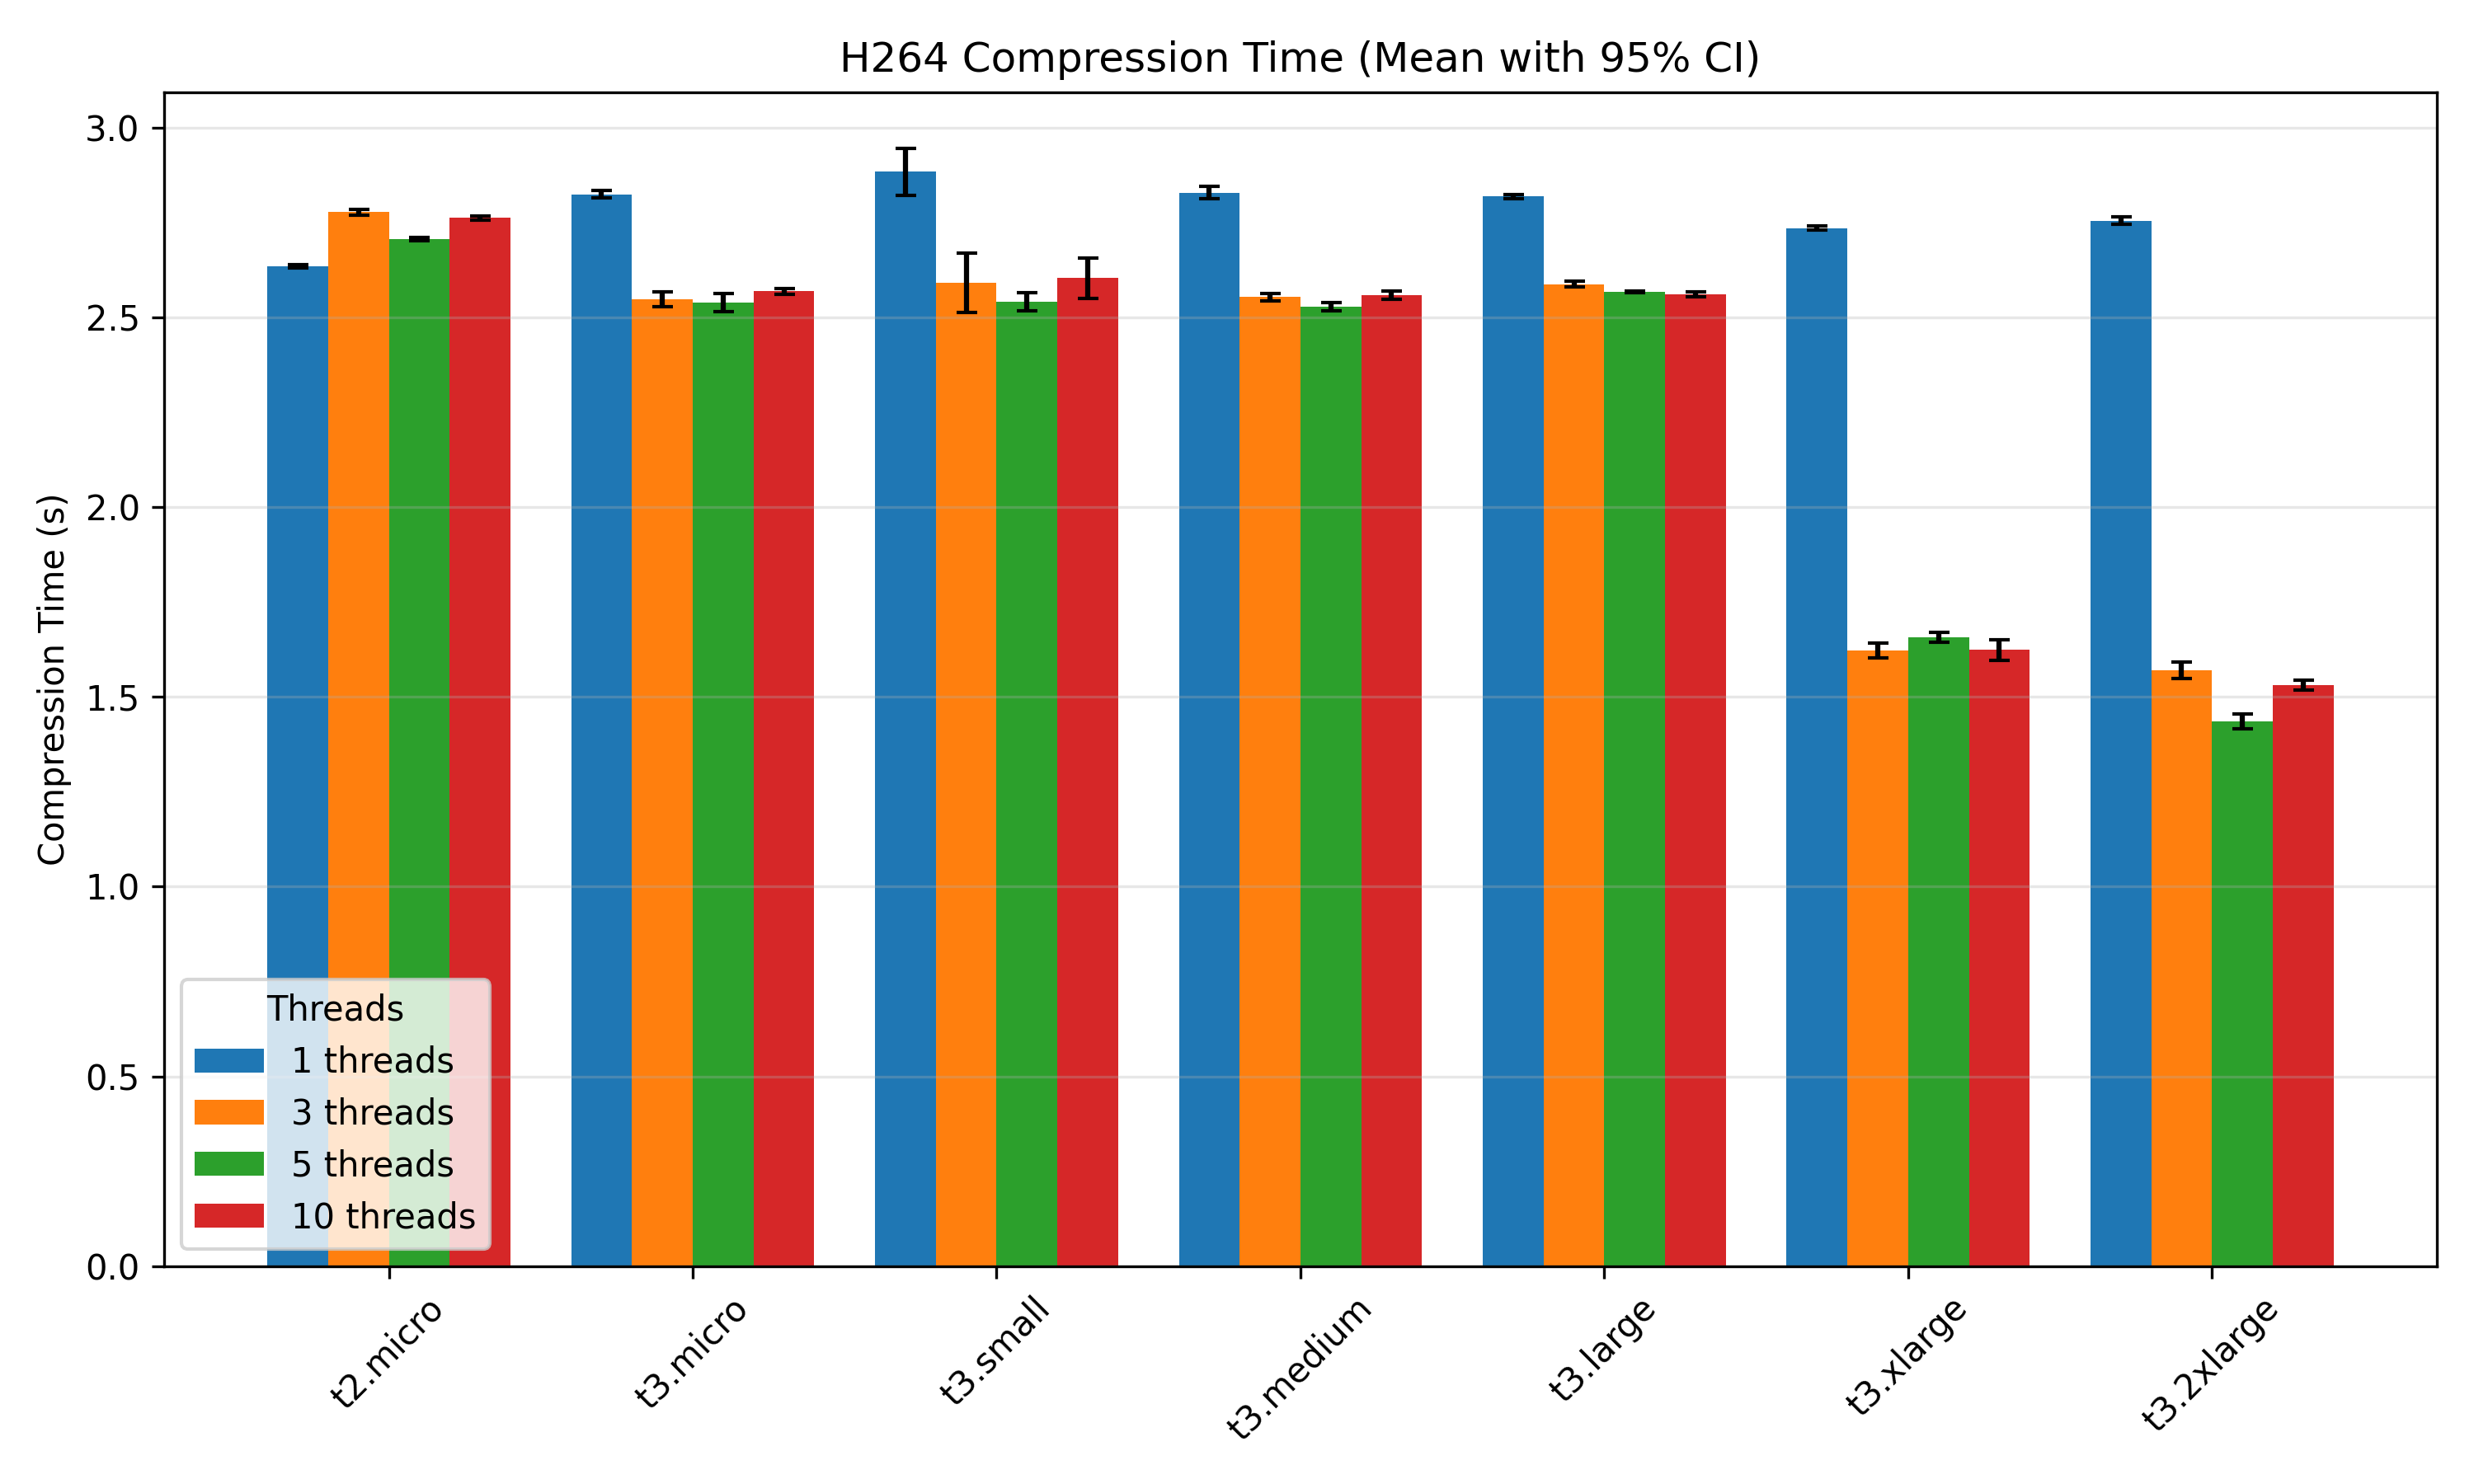
\includegraphics[width=\linewidth]{graphs/bar_chart_time_h264.png}
			\caption{H.264 Codec Performance}
			\label{fig:chart_h264}
		\end{subfigure}
		
		\vspace{0.5cm}
		
		\begin{subfigure}{\columnwidth}
			\centering
			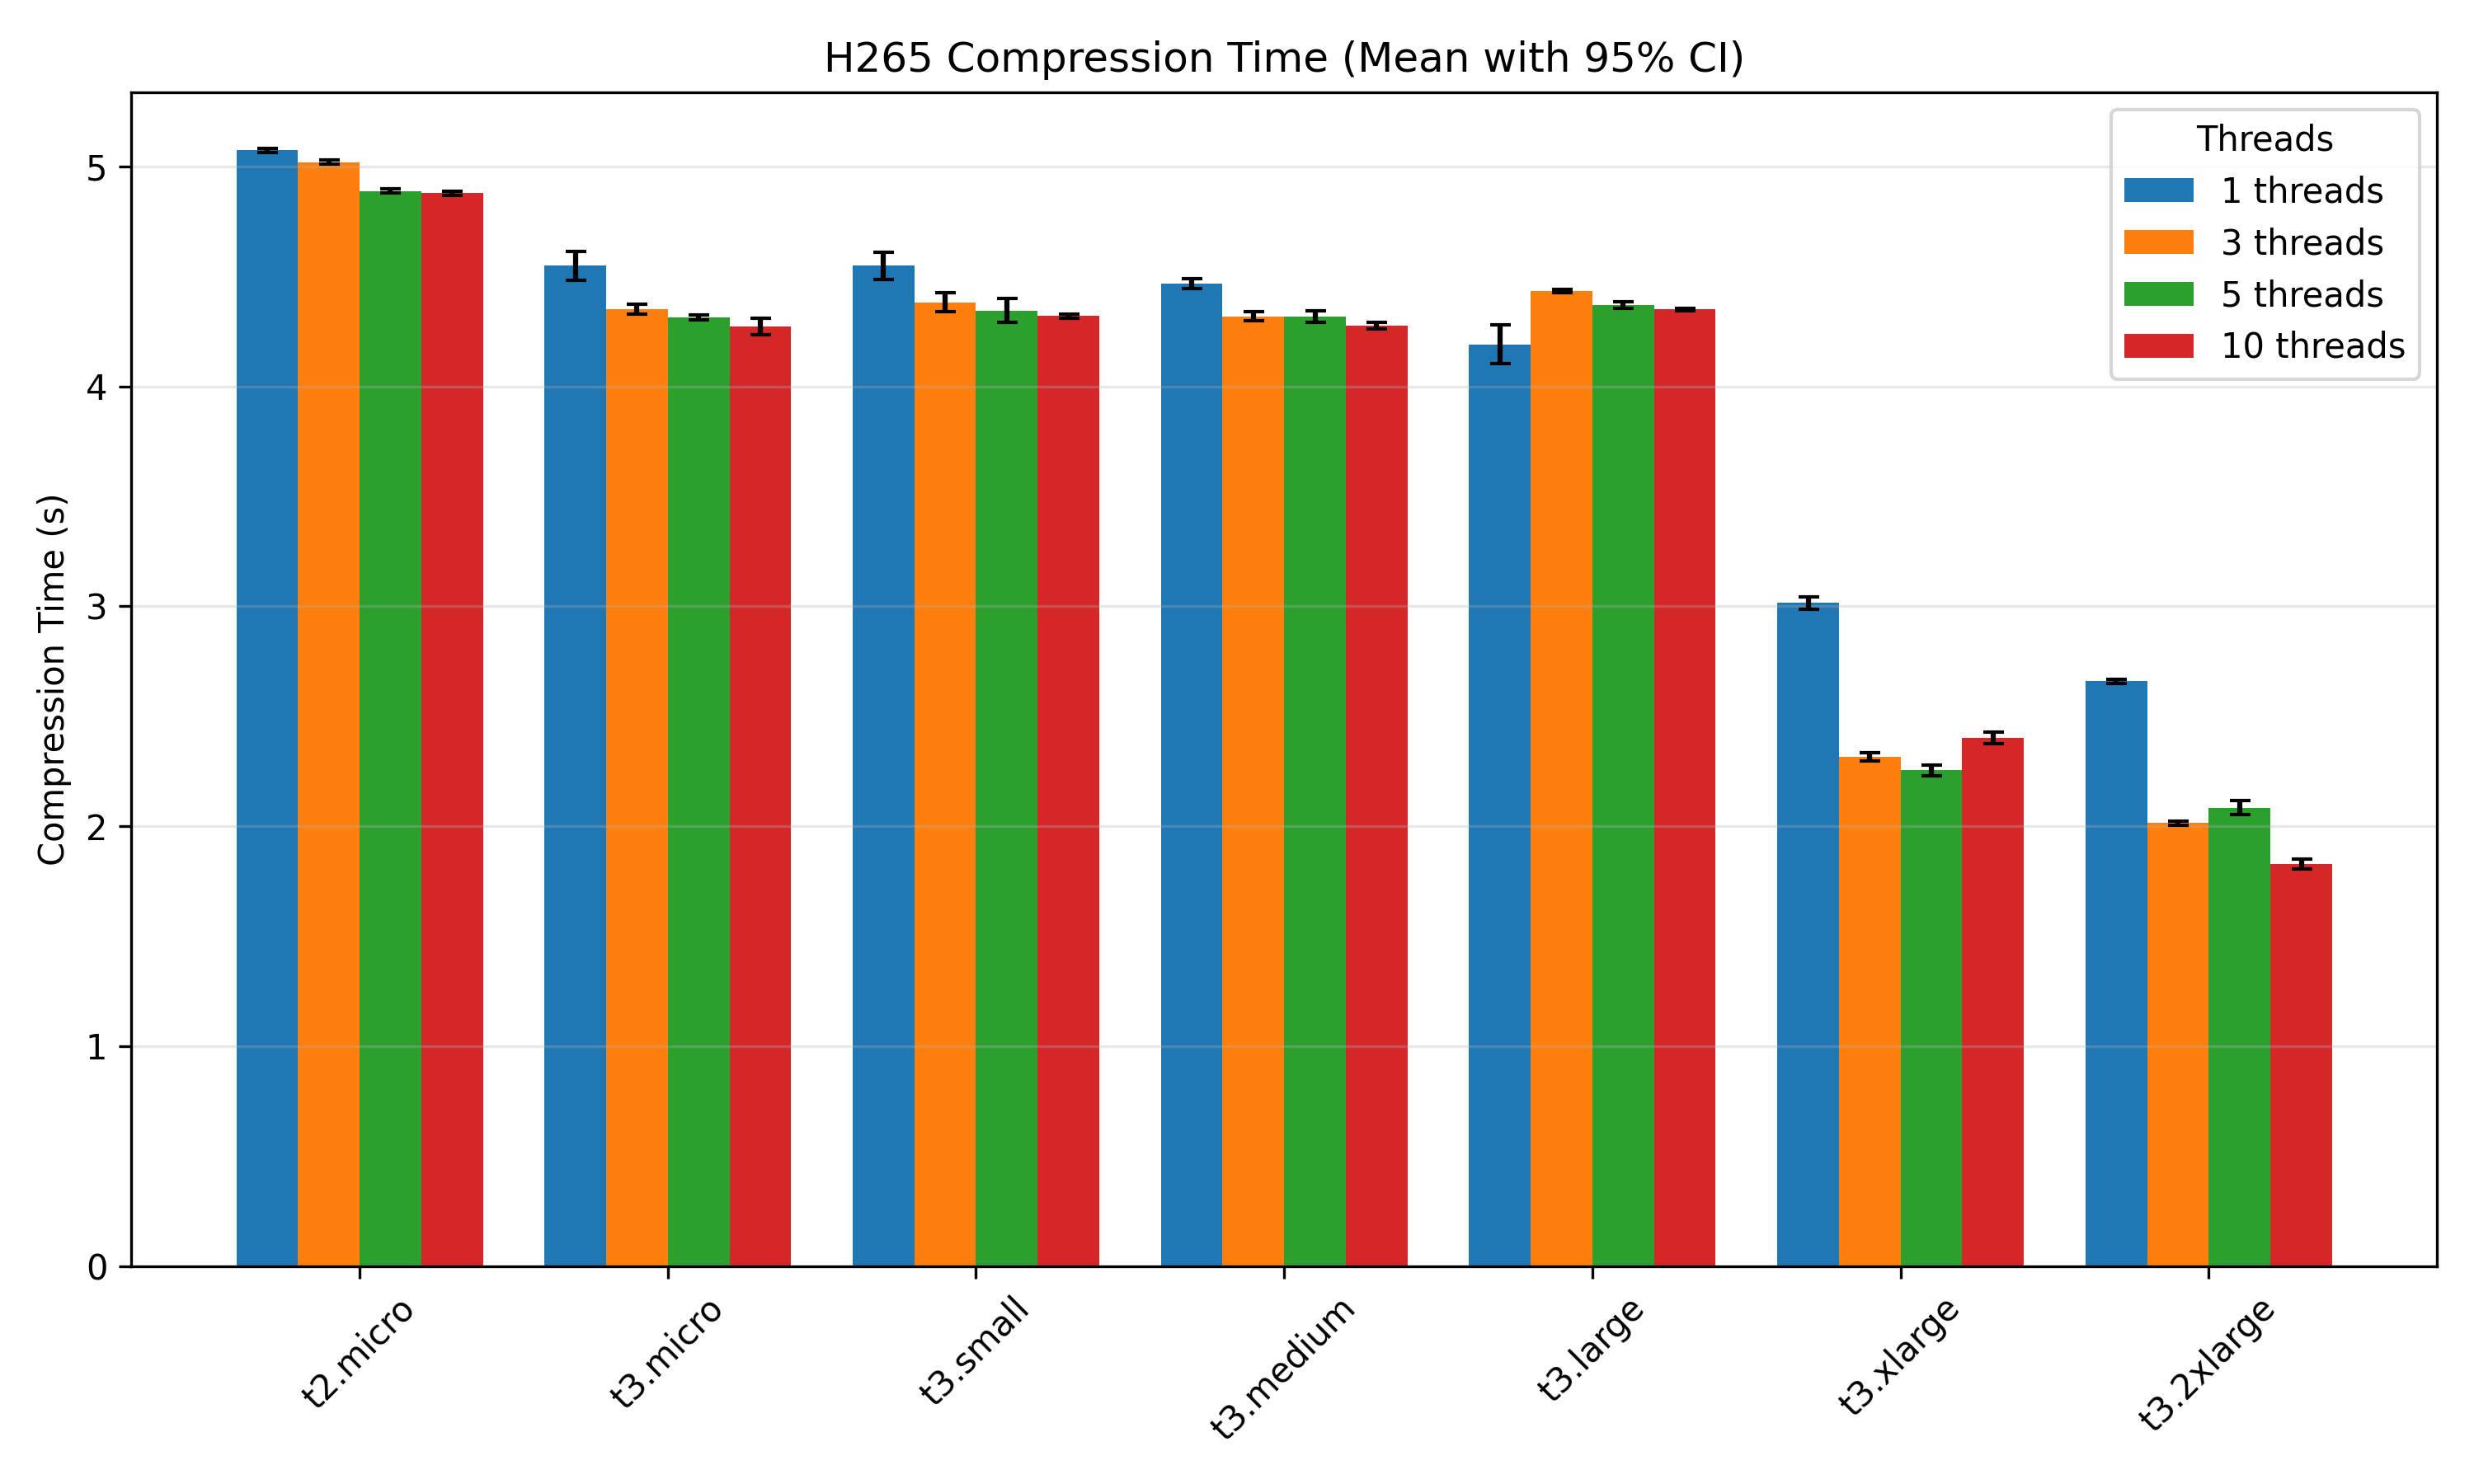
\includegraphics[width=\linewidth]{graphs/bar_chart_time_h265.png}
			\caption{H.265 Codec Performance}
			\label{fig:chart_h265}
		\end{subfigure}
		
		\vspace{0.5cm}
		
		\begin{subfigure}{\columnwidth}
			\centering
			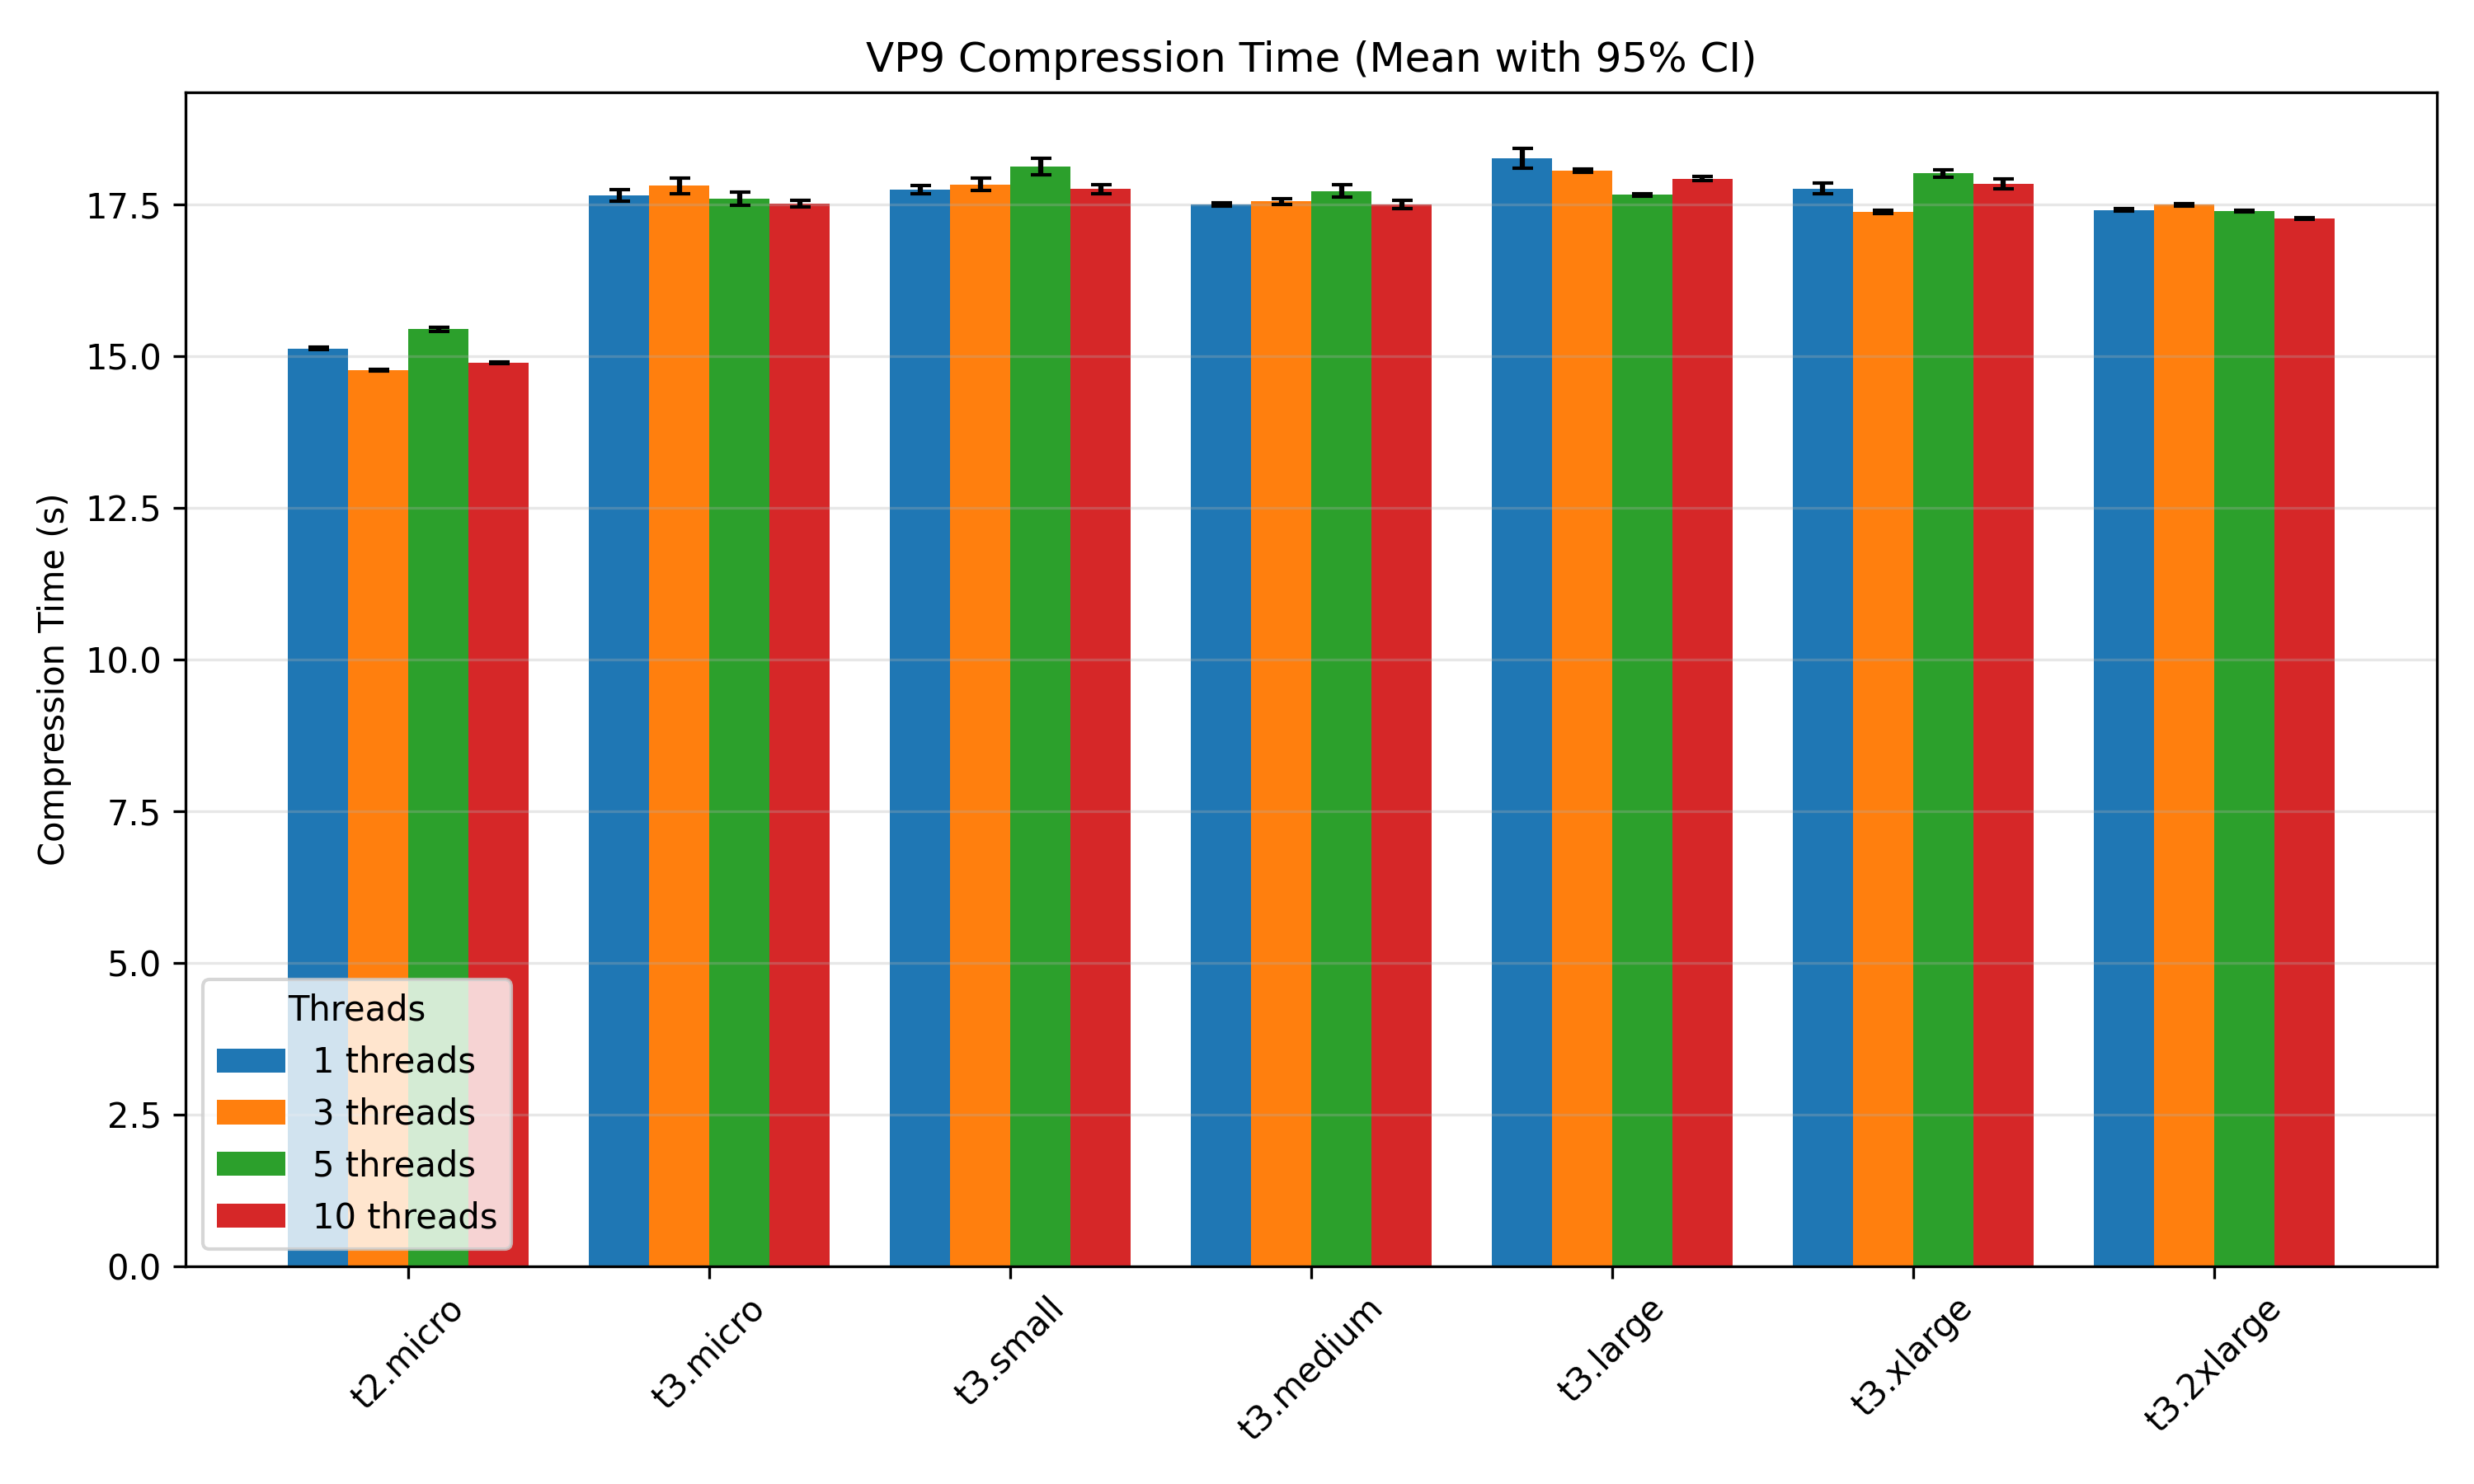
\includegraphics[width=\linewidth]{graphs/bar_chart_time_vp9.png}
			\caption{VP9 Codec Performance}
			\label{fig:chart_vp9}
		\end{subfigure}
		
		\caption{Comparative analysis of median compression time across instance configurations for (a) H.264, (b) H.265, and (c) VP9 codecs. Each panel illustrates performance scaling with varying thread counts.}
		\label{fig:faceted_bar_charts}
	\end{figure}
	
	\textbf{Hierarchical Efficiency Overview:} Figure~\ref{fig:sunburst_efficiency_normalized_overall} presents a normalized Sunburst chart providing a hierarchical overview of encoding efficiency.
	
	\begin{figure*}[ht]
		\centering
		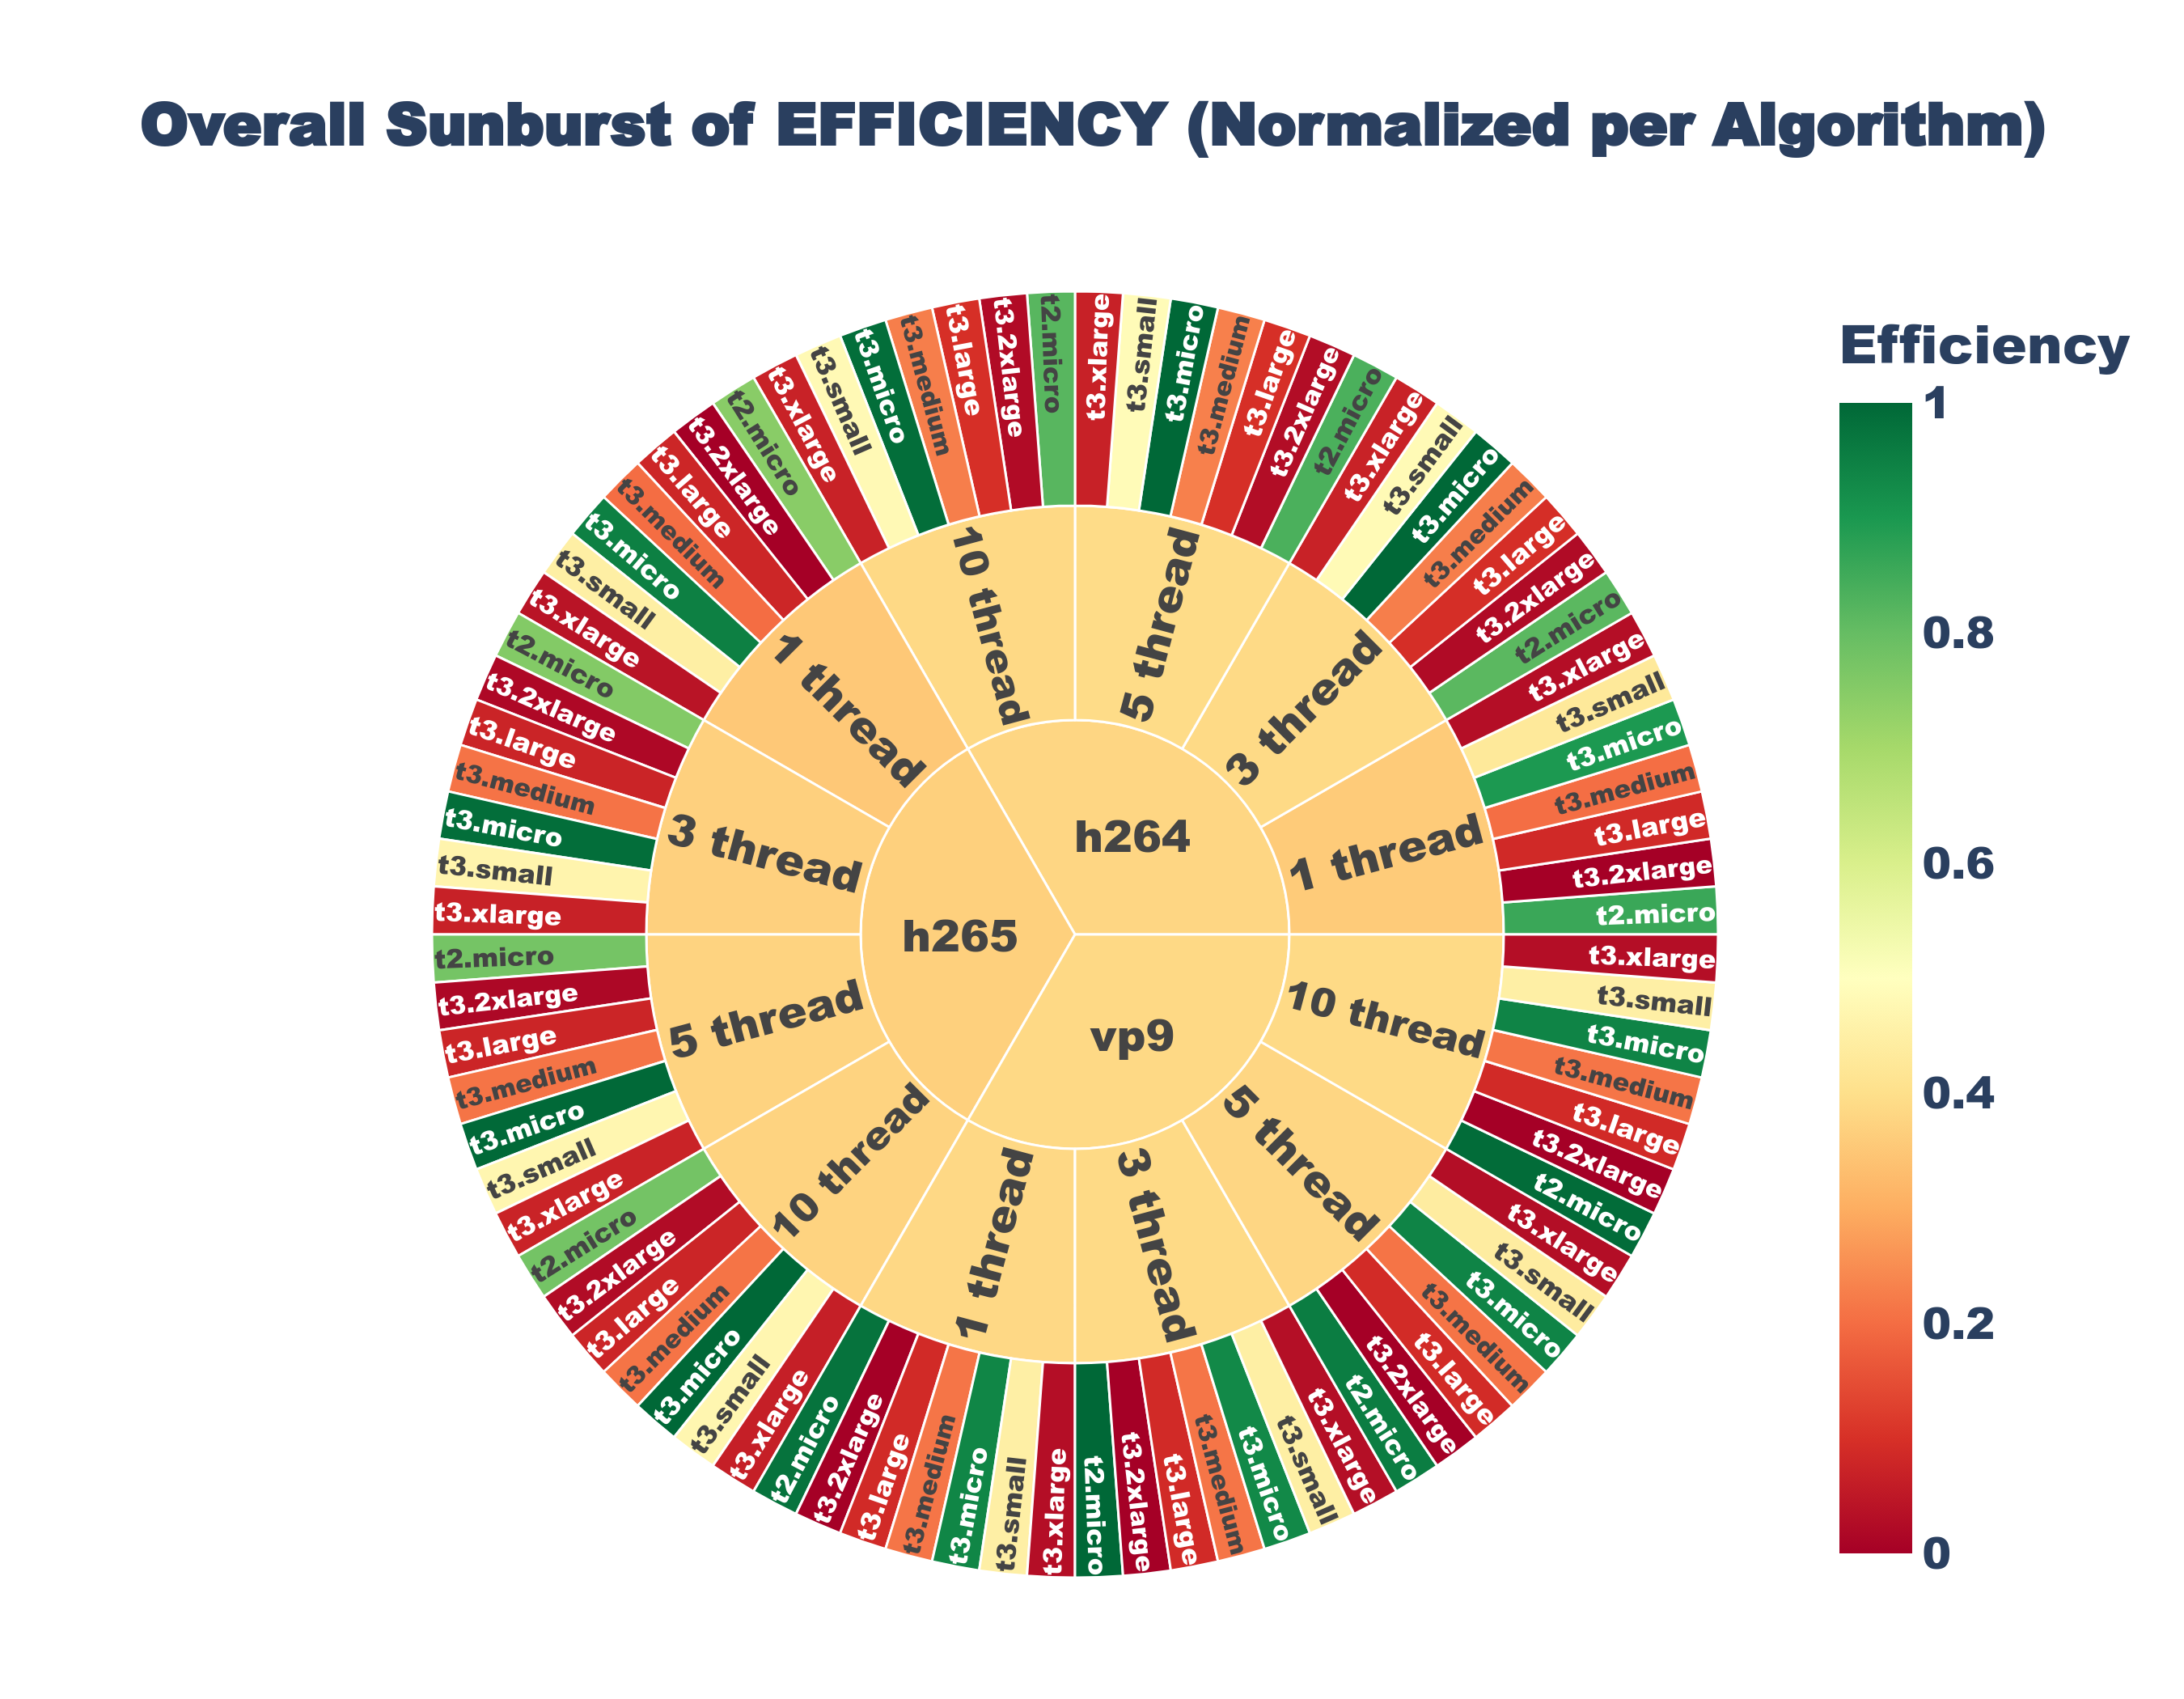
\includegraphics[width=0.7\textwidth]{graphs/sunburst_efficiency_normalized_overall.pdf}
		\caption{Hierarchical visualization of encoding efficiency across all experimental configurations.}
		\label{fig:sunburst_efficiency_normalized_overall}
	\end{figure*}
	
	\textbf{Algorithm-Specific Efficiency Analysis:} Figure~\ref{fig:heatmaps_efficiency} presents heatmaps visualizing median efficiency for each algorithm.
	
	\begin{figure}[htpb]
		\centering
		\begin{subfigure}{\columnwidth}
			\centering
			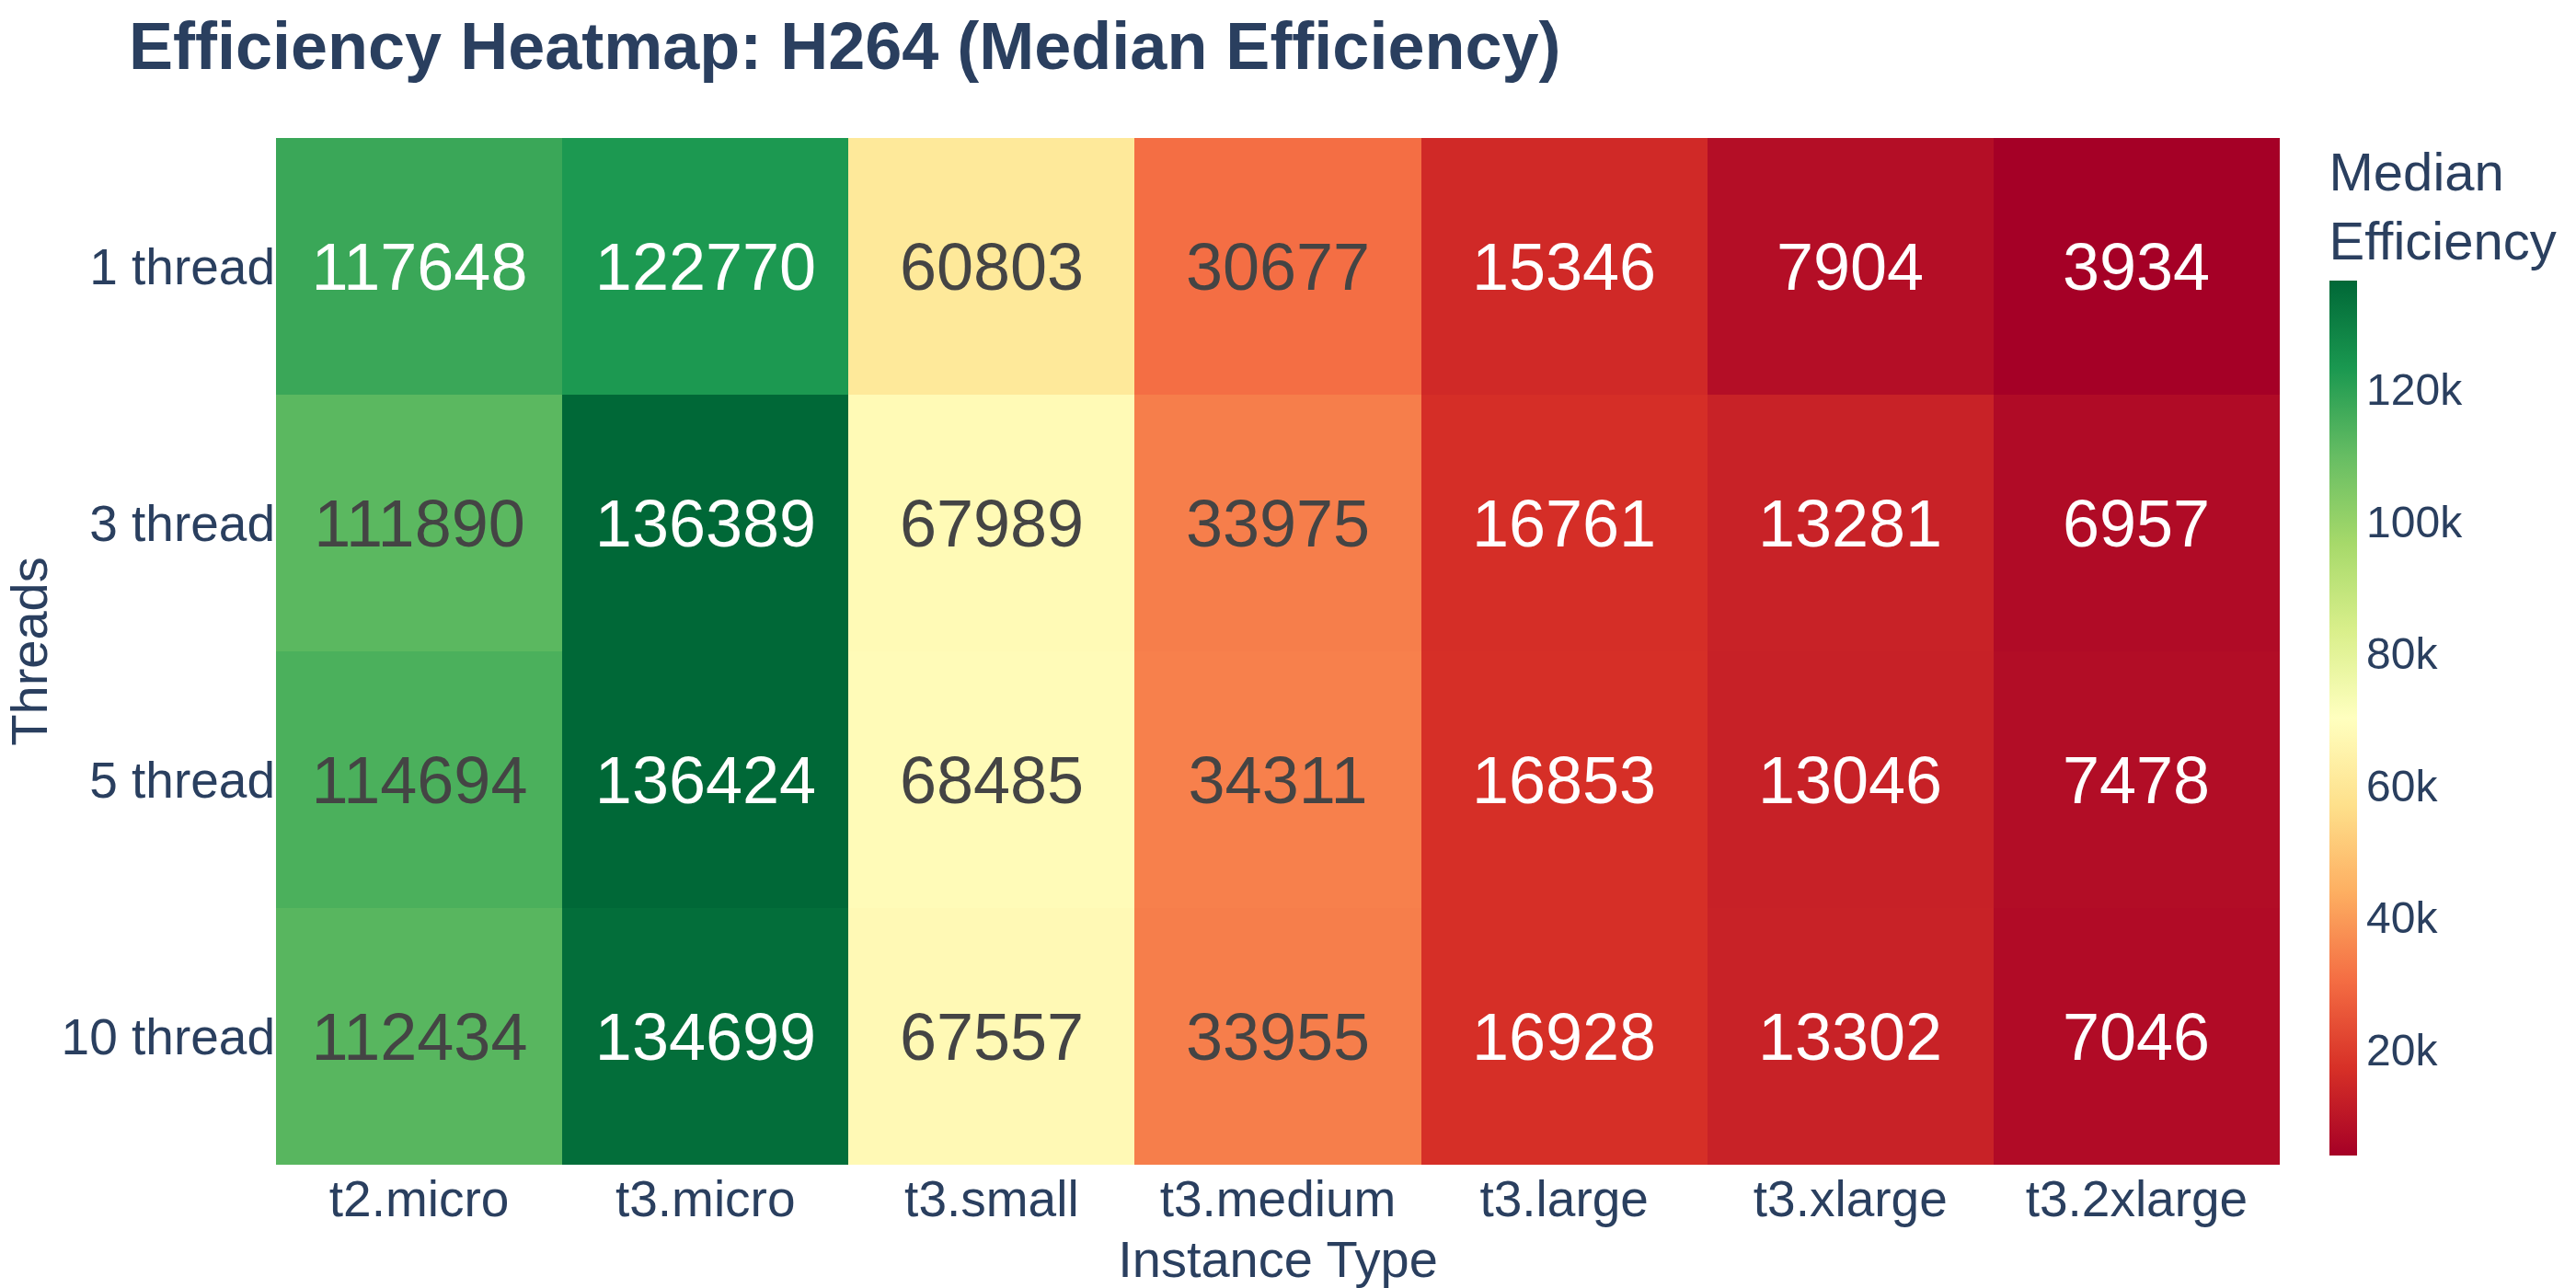
\includegraphics[width=0.98\columnwidth,height=5cm,keepaspectratio]{graphs/heatmap_efficiency_h264.png}
			\caption{H.264 Codec Efficiency}
			\label{fig:h264}
		\end{subfigure}
		\vfill
		\begin{subfigure}{\columnwidth}
			\centering
			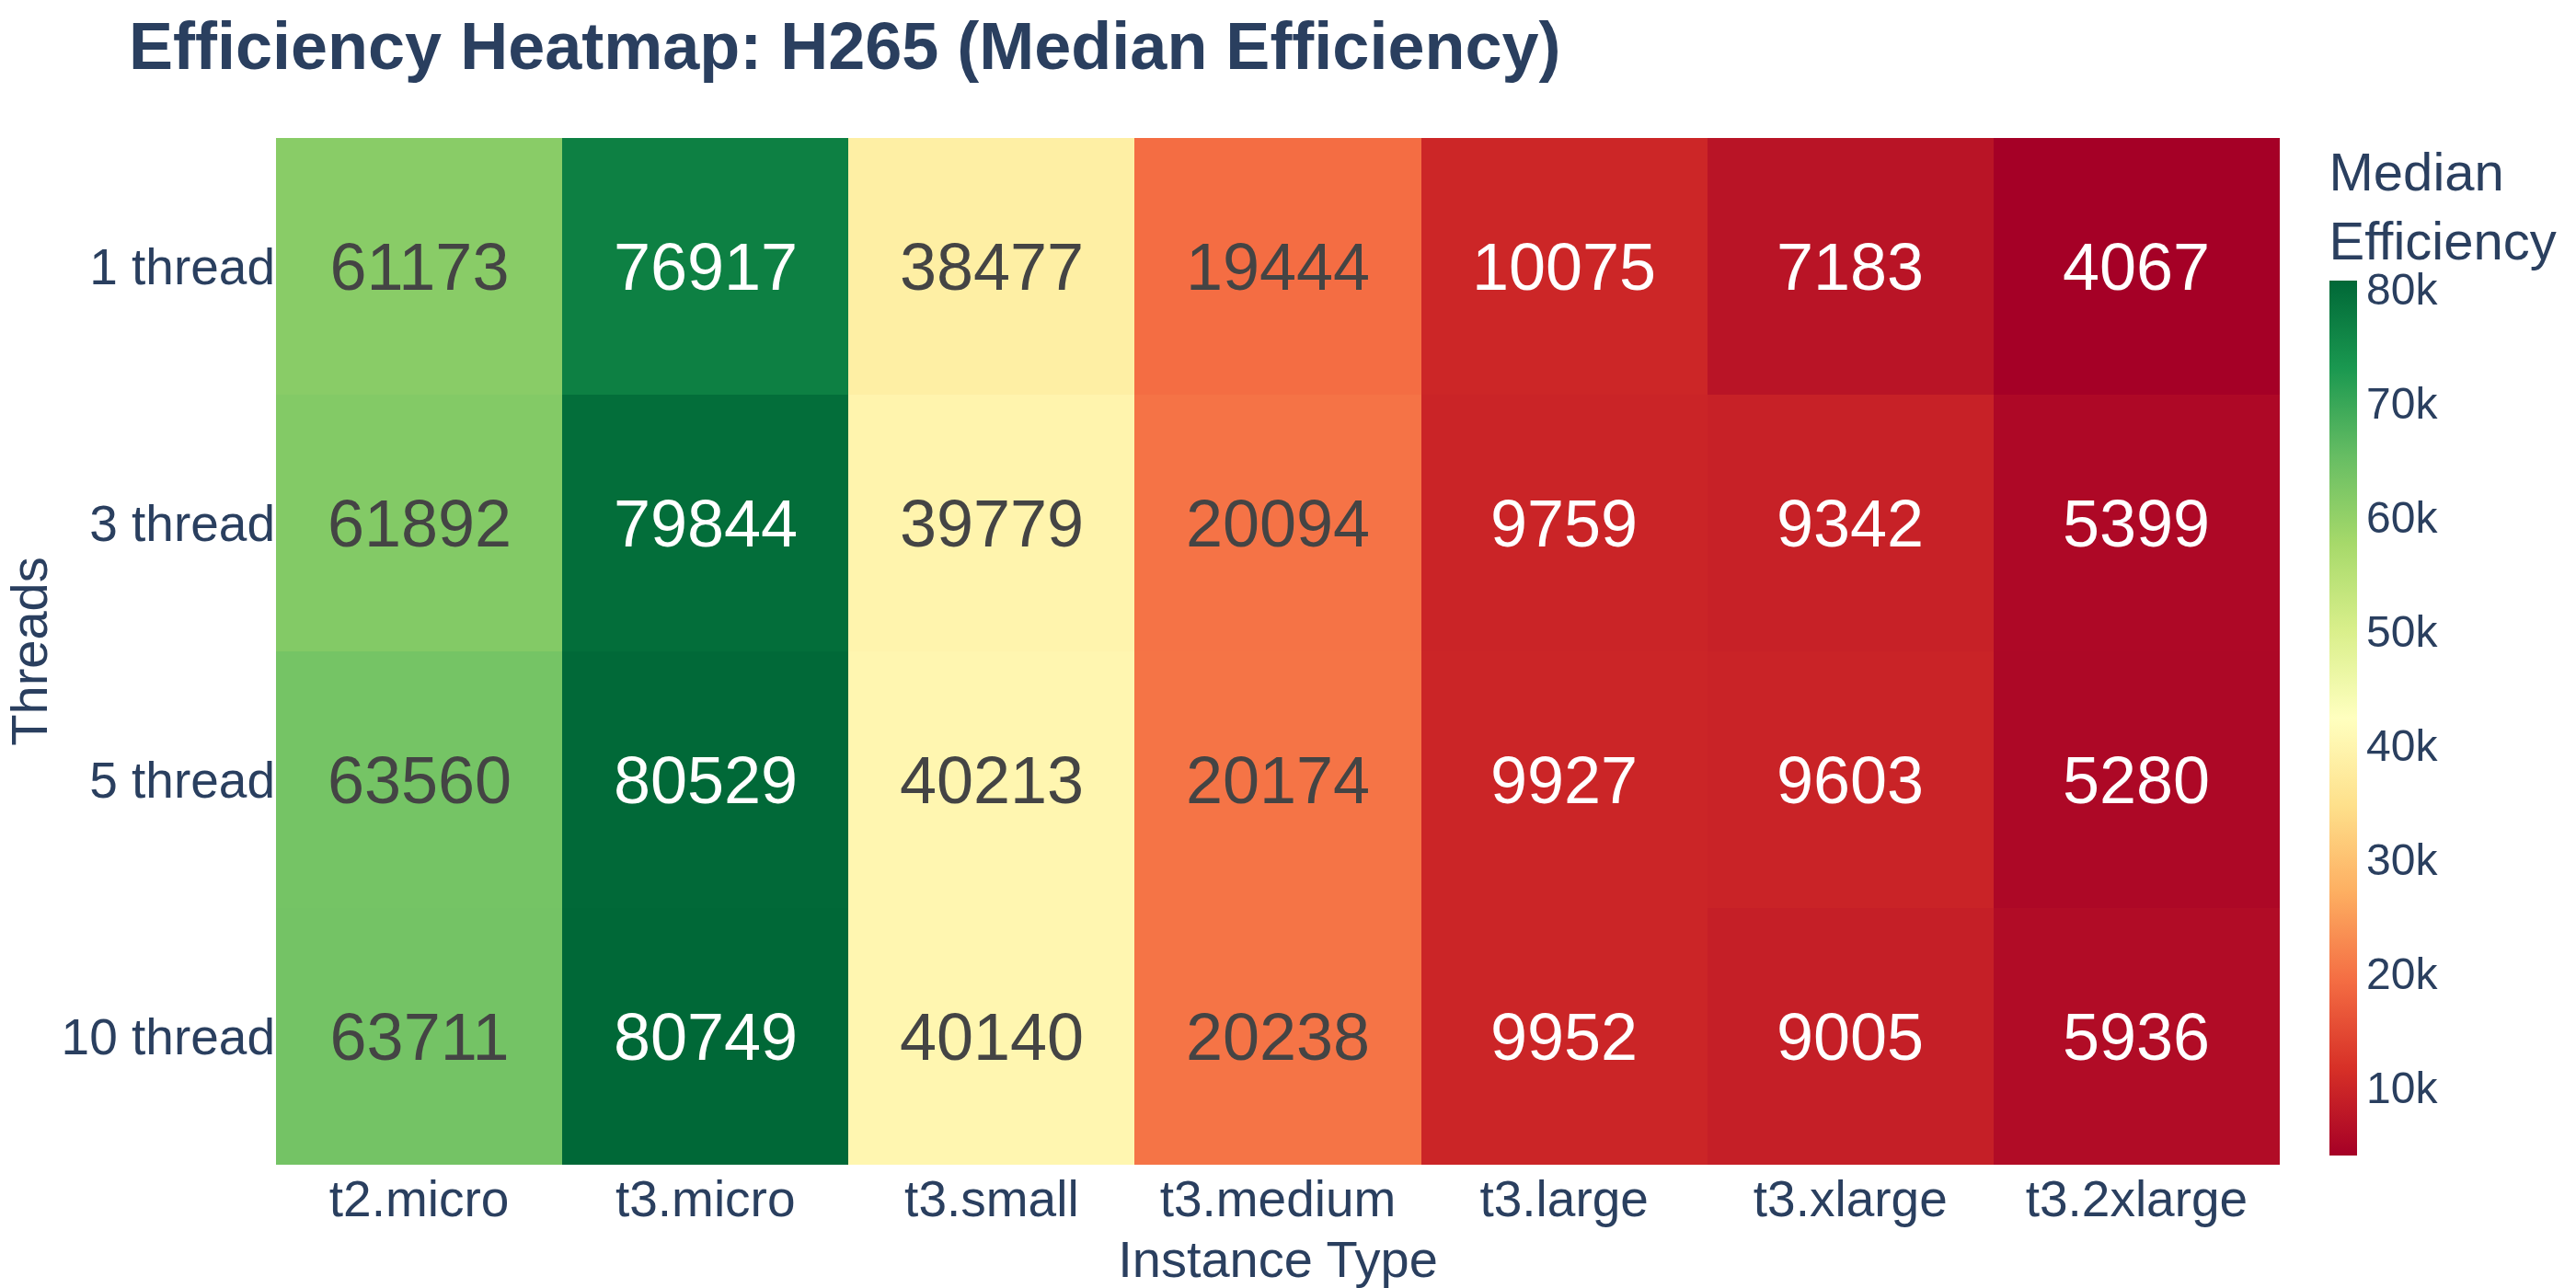
\includegraphics[width=0.98\columnwidth,height=5cm,keepaspectratio]{graphs/heatmap_efficiency_h265.png}
			\caption{H.265 Codec Efficiency}
			\label{fig:h265}
		\end{subfigure}
		\vfill
		\begin{subfigure}{\columnwidth}
			\centering
			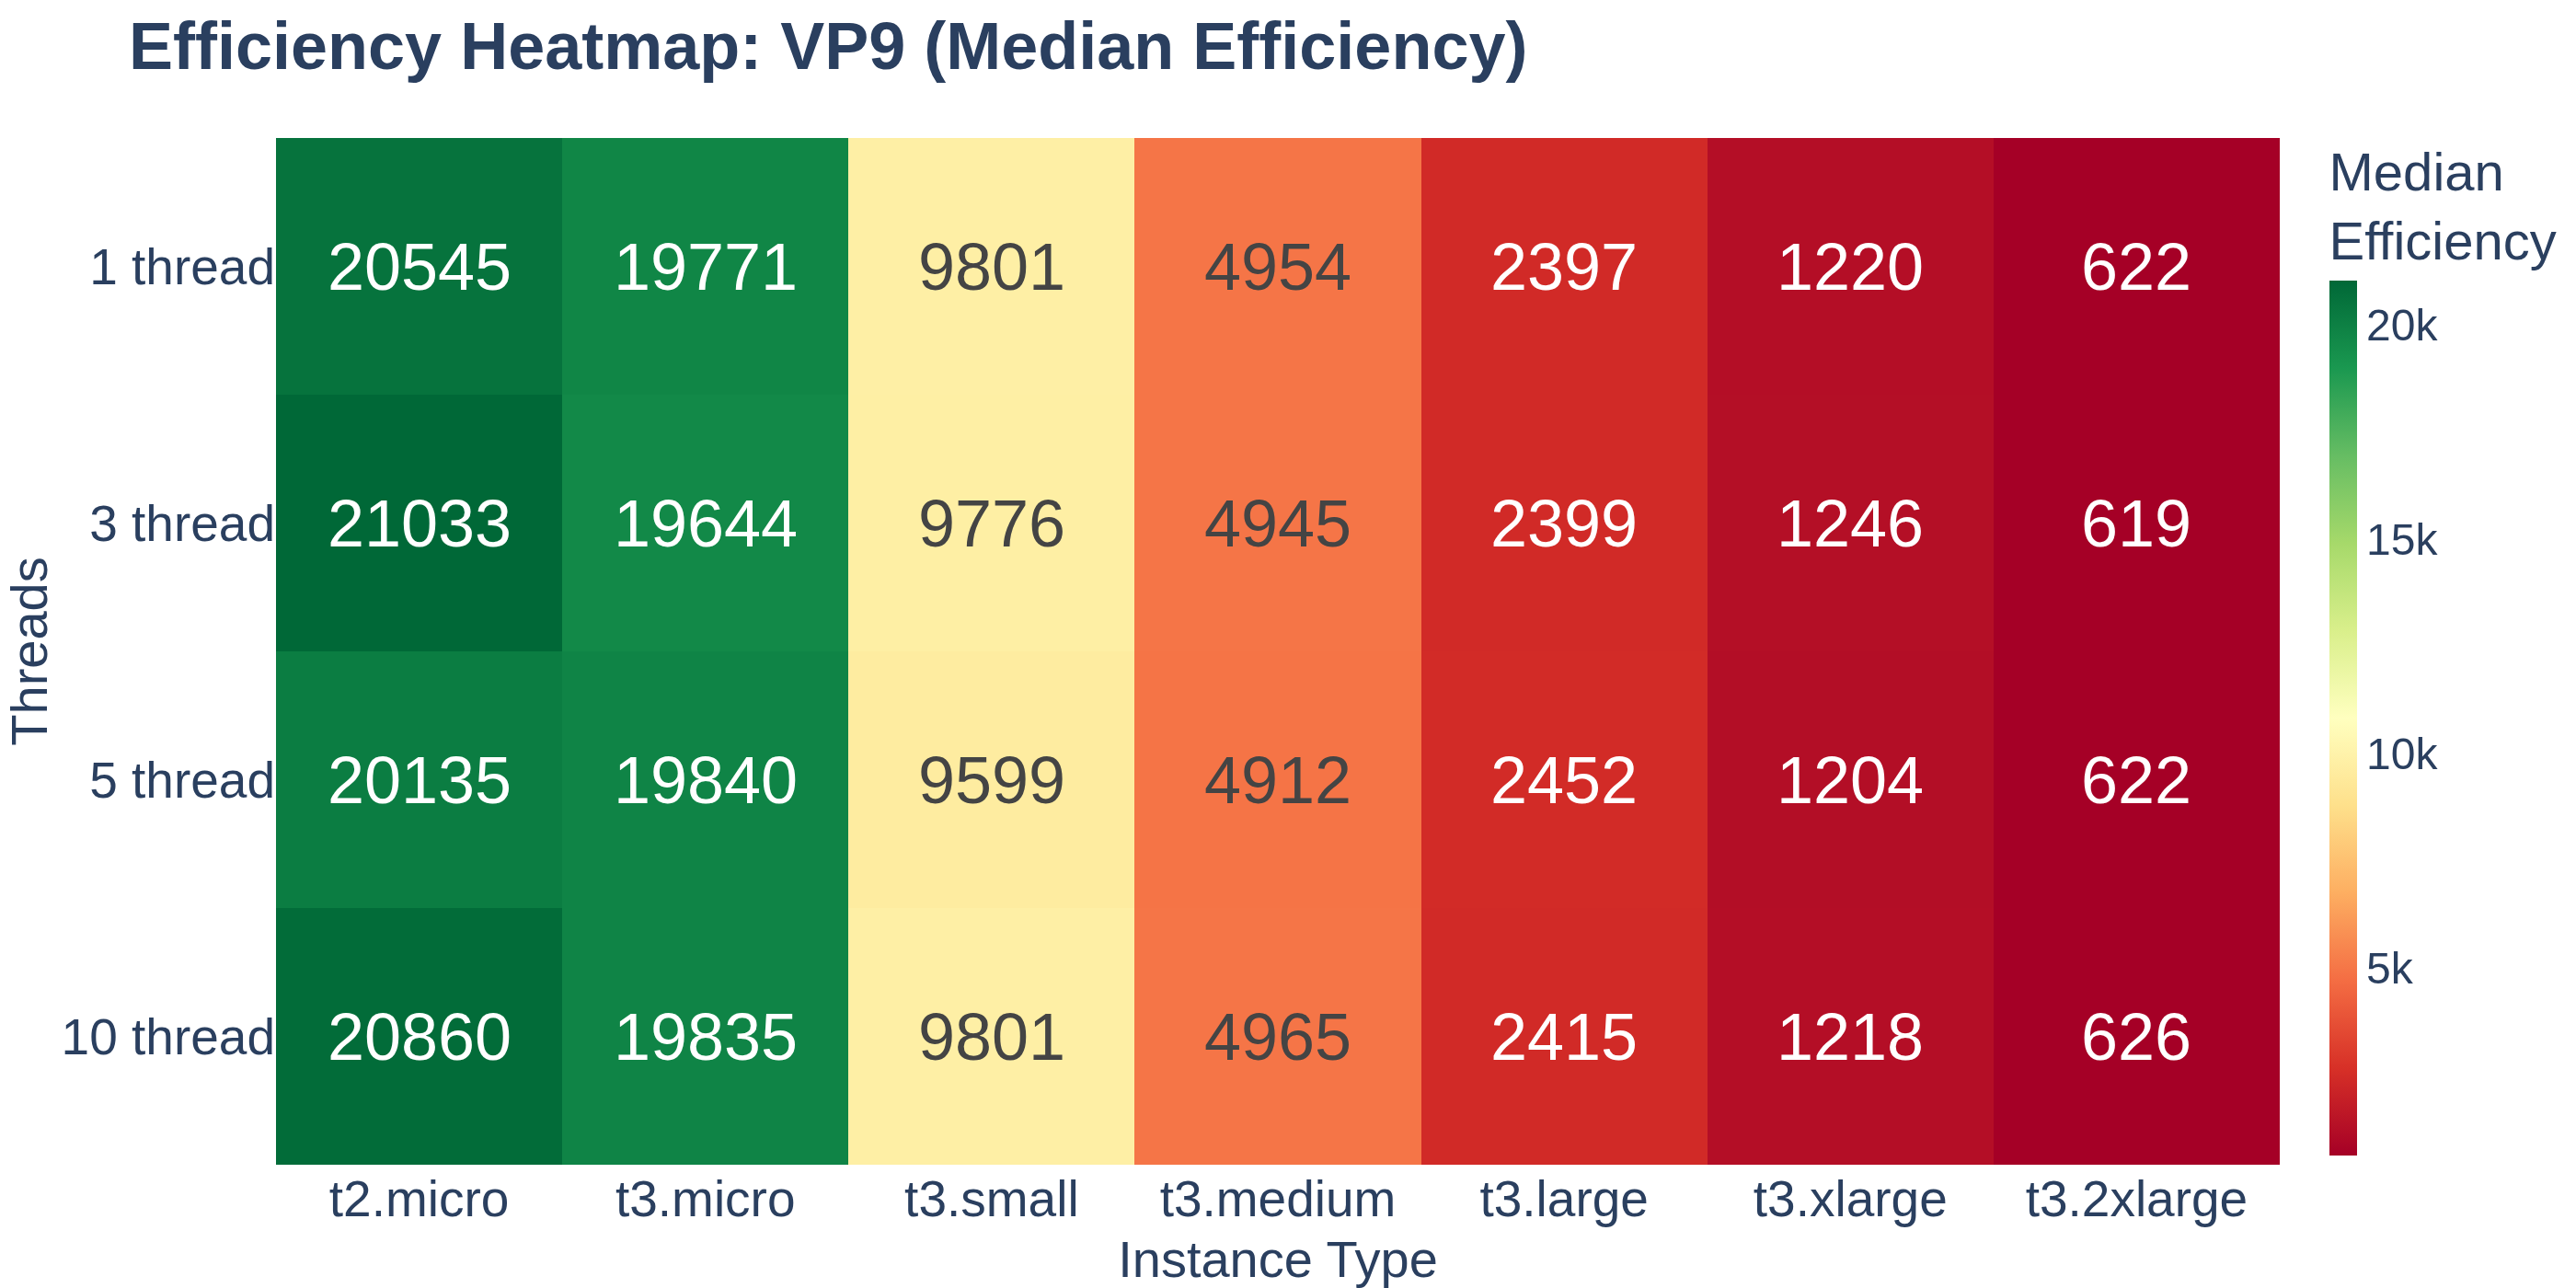
\includegraphics[width=0.98\columnwidth,height=5cm,keepaspectratio]{graphs/heatmap_efficiency_vp9.png}
			\caption{VP9 Codec Efficiency}
			\label{fig:vp9}
		\end{subfigure}
		\caption{Algorithm-specific efficiency analysis through heatmap visualization.}
		\label{fig:heatmaps_efficiency}
	\end{figure}
	
	\subsection{Phase 3 Results: Horizontal vs. Vertical Scaling Analysis}
	\label{results-phase3}
	
	Based on findings identifying \texttt{t3.micro} as most cost-effective, we compared scaling strategies using a 10-minute video workload:
	
	\begin{itemize}
		\item \textbf{Horizontal Scaling:} 10 \texttt{t3.micro} instances processing one-minute segments
		\item \textbf{Vertical Scaling:} Single \texttt{t3.2xlarge} instance processing complete video
		\item \textbf{Baseline:} Single \texttt{t3.micro} instance processing video sequentially
	\end{itemize}
	
	\subsubsection{Two-Phase Analysis Results}
	
	The analysis used two phases to isolate provisioning overhead:
	
	\textbf{Phase 3.1: Dynamic Provisioning} (standard Ubuntu images):
	\begin{itemize}
		\item Setup activities consumed 56.1-75.9\% of total processing time
		\item Vertical scaling completed workload in 3.04 minutes, outperforming horizontal scaling (3.28 minutes) by 7.9\%
		\item Horizontal approach: \$0.00568 vs. \$0.01687 (66.3\% reduction)
	\end{itemize}
	
	\textbf{Phase 3.2: Optimized Provisioning} (custom AMIs):
	\begin{itemize}
		\item Horizontal scaling achieved 1.45 minutes total time — 55.9\% improvement and 1.28× faster than vertical scaling (1.85 minutes)
		\item Costs reduced by 55.8\% to \$0.00251 (75.5\% cost reduction)
		\item Setup time decreased from 2.30 minutes to 0.98 minutes (57.4\% reduction)
	\end{itemize}
	
	\begin{table*}[t]
		\centering
		\caption{Comprehensive comparison of scaling strategies across optimization phases}
		\label{tab:unified_case_study}
		\begin{tabular*}{\textwidth}{l @{\extracolsep{\fill}} | cc | cc | cc}
			\toprule
			& \multicolumn{2}{c|}{\textbf{Serial (1x t3.micro)}} & \multicolumn{2}{c|}{\textbf{Parallel (10x t3.micro)}} & \multicolumn{2}{c}{\textbf{Serial (1x t3.2xlarge)}} \\
			\cmidrule(lr){2-3} \cmidrule(lr){4-5} \cmidrule(lr){6-7}
			\textbf{Metric} & \textbf{Phase 3.1} & \textbf{Phase 3.2} & \textbf{Phase 3.1} & \textbf{Phase 3.2} & \textbf{Phase 3.1} & \textbf{Phase 3.2} \\
			\midrule
			Total Time (min)          & 4.03  & 2.80  & 3.28 & \textbf{1.45} & 3.04 & 1.85 \\
			Setup Overhead (min)      & 2.26  & 1.02  & 2.30 & \textbf{0.98} & 2.31 & 1.11 \\
			Setup Overhead (\%)       & 56.1\% & 36.5\% & 70.2\% & 67.6\% & 75.9\% & 59.7\% \\
			Effective Encoding Time (min) & 1.77  & 1.78  & 0.97 & 0.47 & \textbf{0.73} & 0.74 \\
			\midrule
			Total Cost (USD)          & \$0.00070 & \$0.00048 & \$0.00568 & \textbf{\$0.00251} & \$0.01687 & \$0.01026 \\
			Cost per Minute Video     & \$0.000070 & \$0.000048 & \$0.000568 & \textbf{\$0.000251} & \$0.001687 & \$0.001026 \\
			\midrule \midrule
			\textbf{Time Improvement} & \multicolumn{2}{c|}{30.5\%} & \multicolumn{2}{c|}{\textbf{55.9\%}} & \multicolumn{2}{c}{39.1\%} \\
			\textbf{Cost Reduction}   & \multicolumn{2}{c|}{31.4\%} & \multicolumn{2}{c|}{\textbf{55.8\%}} & \multicolumn{2}{c}{39.2\%} \\
			\bottomrule
		\end{tabular*}
	\end{table*}
	
	\begin{figure}[ht]
		\centering
		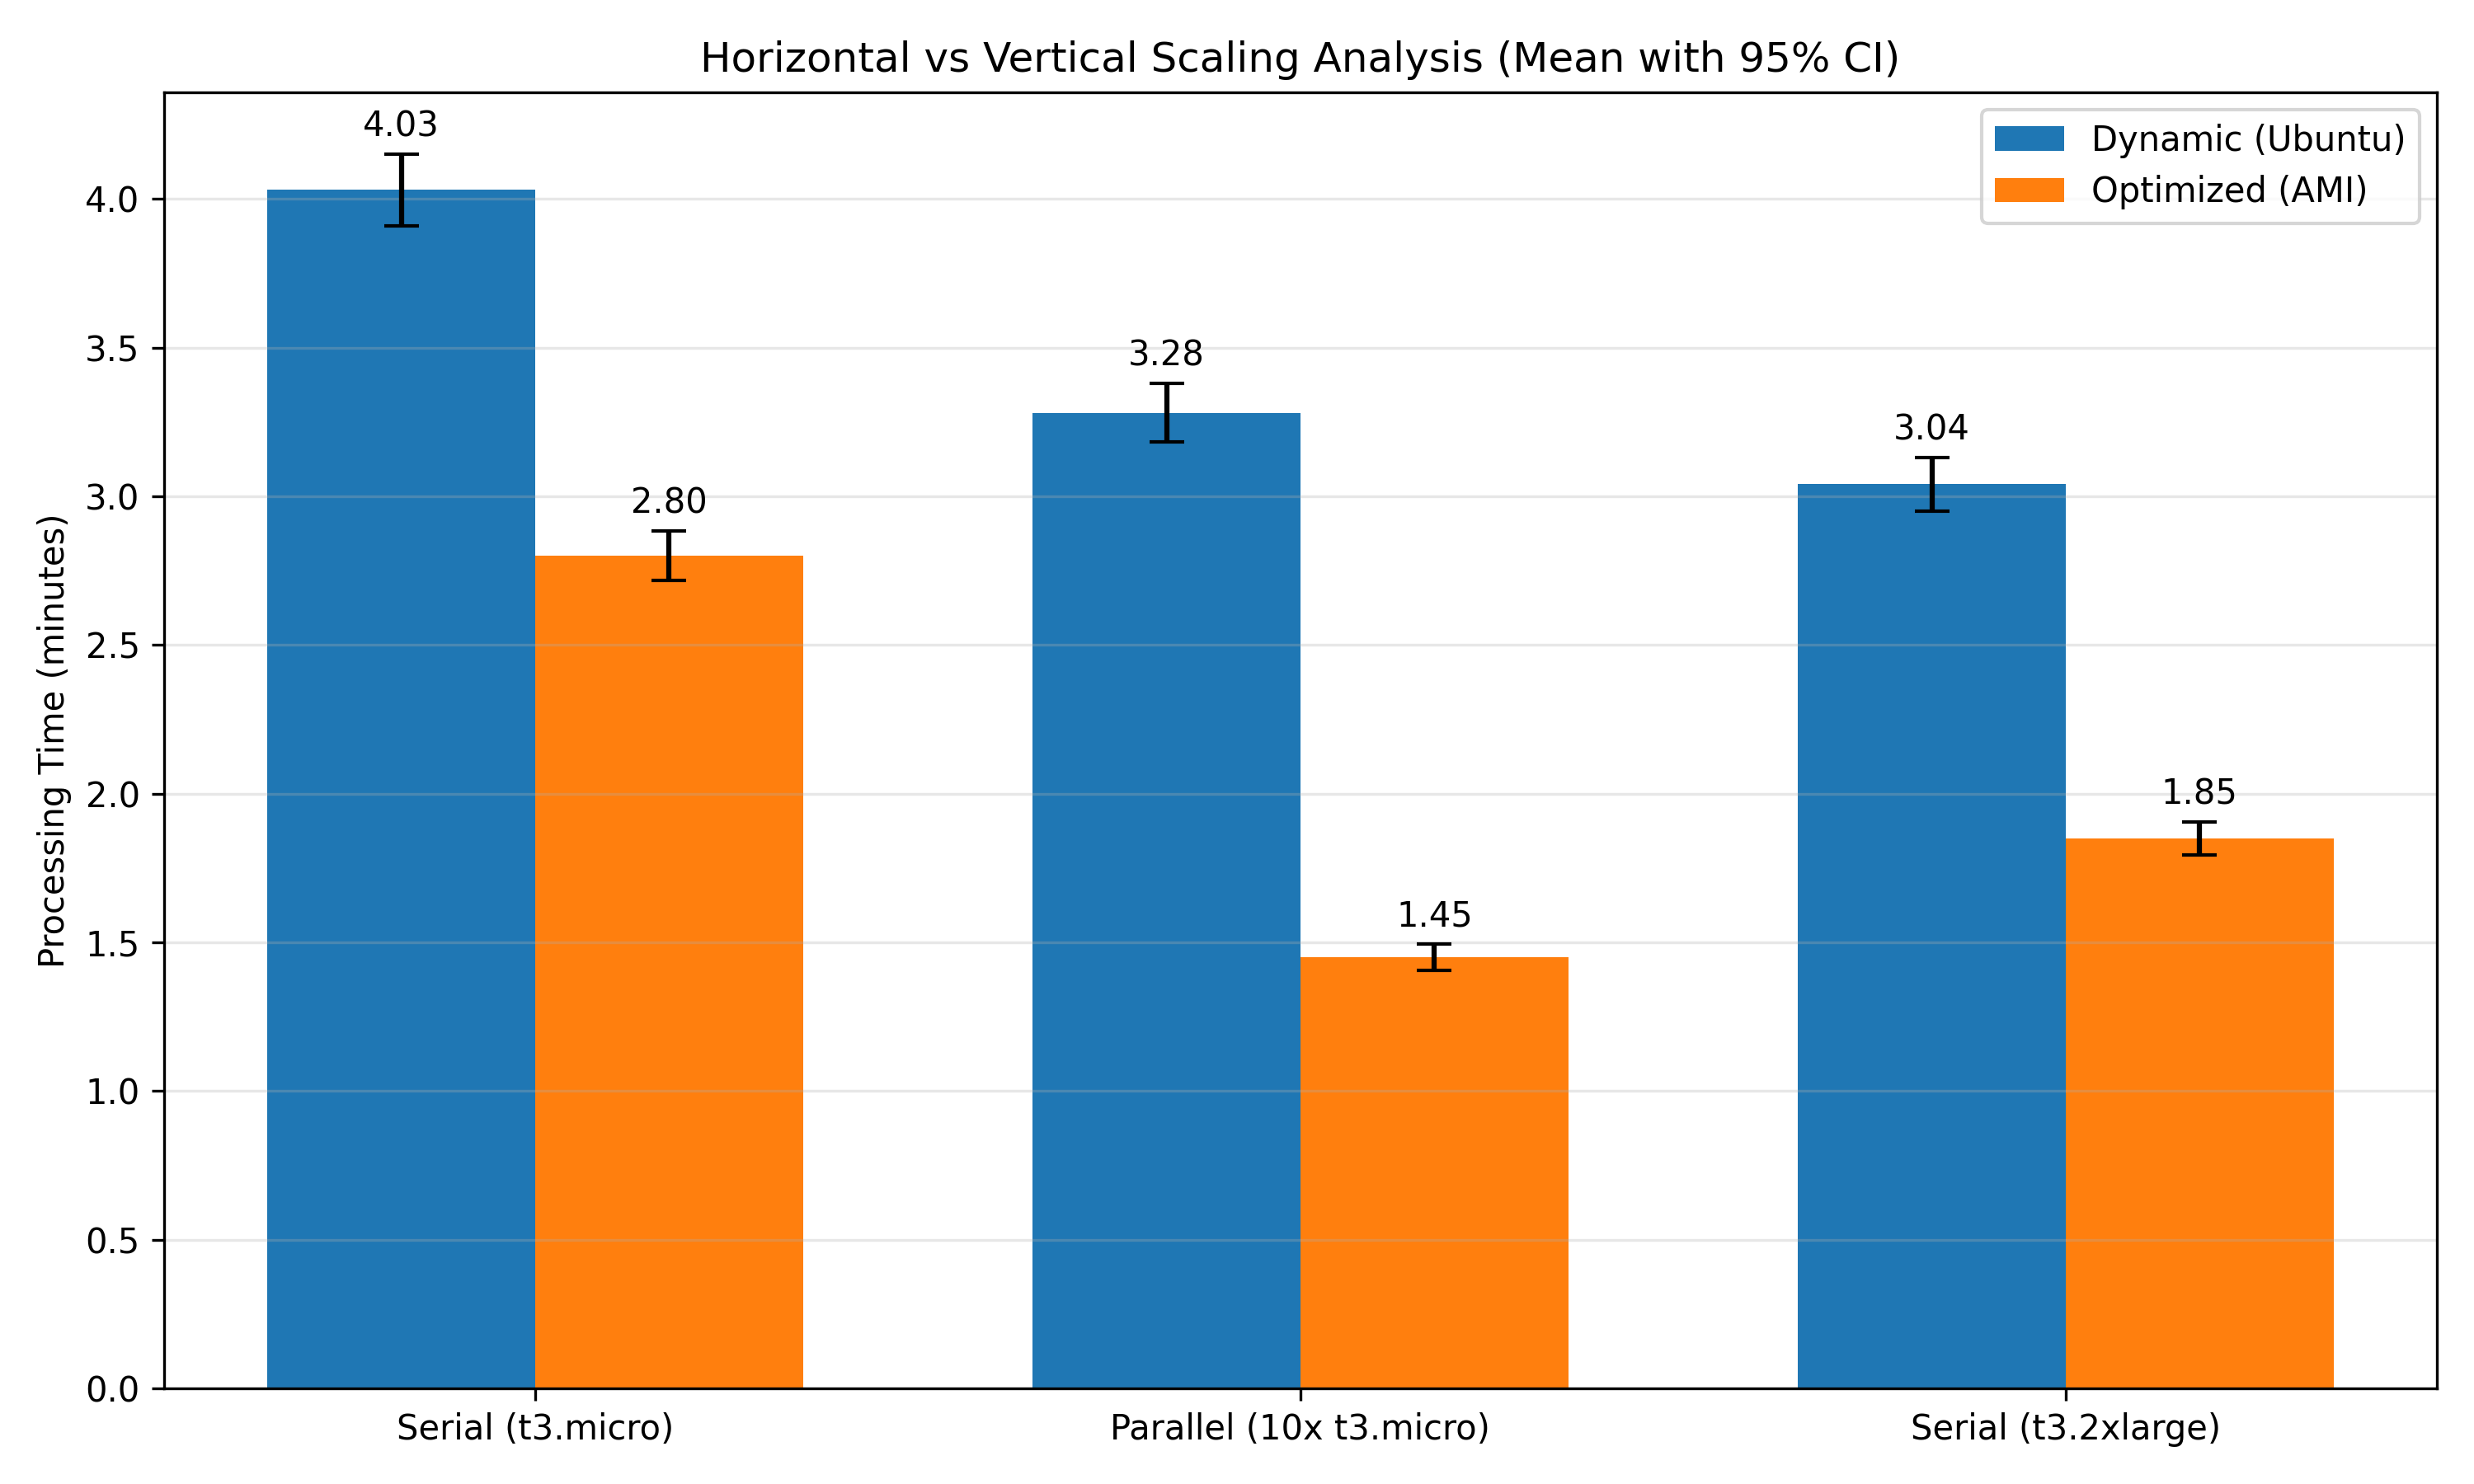
\includegraphics[width=0.5\textwidth]{graphs/comparison_time_cost_dual_axis.png}
		\caption{Performance and cost comparison between dynamic provisioning (Phase 3.1) and optimized provisioning (Phase 3.2).}
		\label{fig:ami_comparison}
	\end{figure}
	
	The results demonstrate that horizontal scaling's advantages can be realized when operational bottlenecks are addressed, achieving 75.5\% cost reduction and 1.28× performance improvement.
	
	\section{Conclusion}
	\label{conclusion}
	
	This study demonstrates that architectural choices impact the cost-efficiency of video encoding in cloud environments. Our empirical analysis shows that smaller burstable instances (t3.micro) achieve up to 20× higher cost-effectiveness despite longer processing times, challenging conventional scaling assumptions. We quantified provisioning overhead, which consumed 70\% of total processing time in unoptimized parallel deployments. By eliminating this overhead through pre-configured machine images, we found that optimized horizontal scaling with t3.micro instances processes videos 1.28× faster while reducing costs by 75.5\% compared to vertical scaling.
	
	These findings have implications for cloud computing research and practice. The results challenge assumptions that raw computational power correlates with economic efficiency and establish provisioning overhead as a factor in distributed system performance. For practice, they indicate that pre-configured images are necessary for parallel encoding architectures, and that horizontal scaling with cost-optimized instances can outperform vertical scaling for divisible video workloads.
	
	Future research could extend this framework to additional media processing workloads, develop intelligent scaling systems that adapt instance counts based on real-time workload characterization, explore fault-tolerant patterns for spot instance utilization, and investigate performance variability in minimal instances. This research provides a foundation for efficient cloud resource utilization in media processing applications.
	\clearpage
	\begin{thebibliography}{00}
		\bibitem{b1} W. Maas, F. Rossi, M. Caggiani, P. Navaux, and A. Lorenzon, ``Investigating cloud instances to achieve optimal trade-offs between performance-cost efficiency,'' \emph{Computing}, vol. 107, no. 1, pp. 82--97, Jan. 2025. doi: 10.1007/s00607-025-01444-9.
		
		\bibitem{b2} P. Álvarez, S. Hernández, J. Fabra, and J. Ezpeleta, ``Cost-driven provisioning and execution of a computing-intensive service on the Amazon EC2,'' \emph{The Computer Journal}, vol. 61, no. 9, pp. 1407--1421, Jan. 2018. doi: 10.1093/comjnl/bxy006.
		
		\bibitem{b3} T. Dancheva, U. Alonso, and M. D. Barton, ``Cloud benchmarking and performance analysis of an HPC application in Amazon EC2,'' \emph{Cluster Computing}, vol. 27, no. 2, pp. 2273--2290, Jun. 2023. doi: 10.1007/s10586-023-04060-4.
		
		\bibitem{b4} L. M. Haji, S. R. M. Zeebaree, O. M. Ahmed, A. B. Sallow, K. Jacksi, and R. R. Zeabri, ``Dynamic Resource Allocation for Distributed Systems and Cloud Computing,'' \emph{Test Engineering and Management}, vol. 83, no. 1, pp. 22417--22426, Jun. 2020.
		
		\bibitem{b5} Z. Ou, H. Zhuang, J. K. Nurminen, A. Ylä-Jääski, and P. Hui, ``Exploiting Hardware Heterogeneity within the Same Instance Type of Amazon EC2,'' in \emph{Proc. 4th USENIX Conf. Hot Topics Cloud Comput.}, Boston, MA, USA, 2012, pp. 4--4.
		
		\bibitem{b6} Z. Ou, H. Zhuang, A. Lukyanenko, J. K. Nurminen, P. Hui, V. V. Mazalov, and A. Ylä-Jääski, ``Is the Same Instance Type Created Equal? Exploiting Heterogeneity of Public Clouds,'' \emph{IEEE Trans. Cloud Comput.}, vol. 1, no. 2, pp. 201--214, Jan. 2013. doi: 10.1109/TCC.2013.12.
		
		\bibitem{b7} B. Farley, A. Juels, V. Varadarajan, T. Ristenpart, K. D. Bowers, and M. M. Swift, ``More for Your Money: Exploiting Performance Heterogeneity in Public Clouds,'' in \emph{Proc. 3rd ACM Symp. Cloud Comput.}, San Jose, CA, USA, 2012, pp. 20:1--20:14. doi: 10.1145/2391229.2391249.
		
		\bibitem{b8} A. Katsenou, X. Wang, D. Schien, and D. Bull, ``Comparative Study of Hardware and Software Power Measurements in Video Compression,'' in \emph{2024 Picture Coding Symp. (PCS)}, Taichung, Taiwan, 2024, pp. 1--5. doi: 10.1109/PCS60826.2024.10566286.
		
		\bibitem{b9} A. Pereira Ferreira and R. O. Sinnott, ``A Performance Evaluation of Containers Running on Managed Kubernetes Services,'' in \emph{2019 IEEE Int. Conf. Cloud Comput. Technol. Sci. (CloudCom)}, Sydney, Australia, 2019, pp. 199--208. doi: 10.1109/CloudCom.2019.00038.
		
		\bibitem{b10} J. Scheuner and P. Leitner, ``Estimating Cloud Application Performance Based on Micro-Benchmark Profiling,'' in \emph{2018 IEEE 11th Int. Conf. Cloud Comput. (CLOUD)}, San Francisco, CA, USA, 2018, pp. 90--97. doi: 10.1109/CLOUD.2018.00019.
		
		\bibitem{b11} S. Ebneyousef and S. Ghazanfari-Rad, ``Cloud Resource Demand Prediction to Achieve Efficient Resource Provisioning,'' in \emph{2022 8th Iranian Conf. Signal Process. Intell. Syst. (ICSPIS)}, Tehran, Iran, 2022, pp. 1--6. doi: 10.1109/ICSPIS56952.2022.10043900.
		
		\bibitem{b12} T. S. Nikoui, A. Balador, A. M. Rahmani, and Z. Bakhshi, ``Cost-Aware Task Scheduling in Fog-Cloud Environment,'' in \emph{2020 CSI/CPSSI Int. Symp. Real-Time Embedded Syst. Technol. (RTEST)}, Tehran, Iran, 2020, pp. 1--8. doi: 10.1109/RTEST49666.2020.9140118.
		
		\bibitem{b13} Y. Yang and H. Casanova, ``RUMR: Robust Scheduling for Divisible Workloads,'' in \emph{Proc. 12th IEEE Int. Symp. High Perform. Distrib. Comput.}, Seattle, WA, USA, 2003, pp. 114--123. doi: 10.1109/HPDC.2003.1210021.
		
		\bibitem{b14} J. Praveenchandar and A. Tamilarasi, ``Resource Allocation Using Phase Change Hyper Switching Algorithm in the Cloud Environment,'' \emph{Intell. Autom. Soft Comput.}, vol. 34, no. 3, pp. 1839--1850, Aug. 2022. doi: 10.32604/iasc.2022.026354.
		
		\bibitem{b15} R. Rosado, O. Santos, F. Oliveira, L. Silva, G. Sanchez, I. Storch, D. Palomino, and L. Agostini, ``A Coding-Efficiency-Aware Fast Heuristic for VVC Intra-Frame Prediction Targeting 360° Videos,'' in \emph{Proc. 30th Brazilian Symp. Multimedia Web}, Juiz de Fora, Brazil, 2024, pp. 355--359. doi: 10.5753/webmedia.2024.243128.
		
		\bibitem{b16} L. Araújo, A. Duarte, G. Correa, B. Zatt, and D. Palomino, ``Fast ISP Mode Decision for the Versatile Video Coding Intra Prediction Using Machine Learning,'' in \emph{Proc. 30th Brazilian Symp. Multimedia Web}, Juiz de Fora, Brazil, 2024, pp. 162--170. doi: 10.5753/webmedia.2024.243129.
		
		\bibitem{b17} A. Mahida, ``Comprehensive Review on Optimizing Resource Allocation in Cloud Computing for Cost Efficiency,'' \emph{J. Artif. Intell. Cloud Comput.}, vol. 1, no. 2, pp. 1--4, May 2022. doi: 10.47363/JAICC/2022(1)232.
		
		\bibitem{b18} O. Alzakholi, L. M. Haji, H. M. Shukur, R. R. Zebari, S. M. Abas, and M. Sadeeq, ``Comparison Among Cloud Technologies and Cloud Performance,'' \emph{J. Appl. Sci. Technol. Trends}, vol. 1, no. 1, pp. 40--47, Apr. 2020. doi: 10.38094/jastt1219.
		
		\bibitem{b19} P. H. G. Silva, ``Analysis of SPOT Instance Pricing for Cost Minimization in a Multi-Cloud Context'' (In Portuguese), M.S. dissertation, Univ. Federal Pernambuco, Recife, Brazil, 2025.
		
		\bibitem{b20} F. Jiang, K. Ferriter, and C. Castillo, ``A Cloud-Agnostic Framework to Enable Cost-Aware Scheduling of Applications in a Multi-Cloud Environment,'' in \emph{2020 IEEE/IFIP Network Operations and Management Symposium (NOMS)}, Budapest, Hungary, 2020, pp. 1--9. doi: 10.1109/NOMS47738.2020.9110325.
		
	\end{thebibliography}
	
	\clearpage
	Appendix
	\section{Reproducibility and Data Availability}
	
	To ensure complete methodological transparency and enable independent verification of our findings, all experimental artifacts associated with this investigation have been made publicly accessible. This includes the complete instrumentation suite for instance provisioning, hardware verification, experimental orchestration, and data analysis, alongside comprehensive raw and aggregated datasets in standardized CSV format. These research artifacts are maintained in a public repository to facilitate scientific reproducibility and community validation.
	
	
\end{document}